\documentclass{article}
\usepackage[margin = 1in]{geometry}
\usepackage[table]{xcolor}
\usepackage{amsmath,amsthm,amsfonts,dsfont,mathtools,float,setspace, booktabs, algorithm,tcolorbox,xparse,colortbl,longtable,array,multirow,wrapfig,float,pdflscape,tabu, setspace, threeparttable,threeparttablex,makecell, pdfpages, url}
\usepackage{natbib}
\usepackage{lineno}[displaymath, mathlines]
\usepackage[normalem]{ulem}
\usepackage[english]{babel}
\bibliographystyle{plainnat}

\DeclarePairedDelimiter{\ceil}{\lceil}{\rceil}
\DeclarePairedDelimiter\floor{\lfloor}{\rfloor}
\newtheorem{theorem}{Theorem}
\newtheorem{lemma}[theorem]{Lemma}
\newtheorem{refproof}{Proof}
\author{Adam Elder}
\newcommand{\bs}{\boldsymbol}
\newcommand{\sh}{\textcolor{red}}
\newcommand{\pr}{\text{Pr}}
\newcommand{\vmat}{\Sigma}
\newcommand{\indep}{\raisebox{0.05em}{\rotatebox[origin=c]{90}{$\models$}}}
\usepackage[mathscr]{euscript}
\usepackage{algorithm}
\usepackage[noend]{algpseudocode}
\definecolor{Gray}{gray}{0.95}
\newcommand{\rvo}{X}
\newcommand{\norm}{f}
\newcommand{\rvoo}{x}
\newcommand{\disto}{P}
\newcommand{\tst}{\hat{\boldsymbol{t}}}
\newcommand{\rvt}{Y}
\newcommand{\rvv}{Z}
\newcommand{\nrvs}{Y_\Sigma}
\newcommand{\nrvi}{Y_I}
\newcommand{\distv}{Q}
\newcommand{\Gammaf}{\Gamma_{\Sigma}}
\newcommand{\Gammafe}{\Gamma_{\hat{\Sigma}}}
\newcommand{\pf}{\Phi}
\newcommand{\gi}{\Gamma}
\newcommand{\gamestz}{\Gamma(\hat{\rvv}, \hat{\Sigma})}
\newcommand{\gamestp}{\Gamma(\sqrt{n}\hat{\boldsymbol{\psi}}, \hat{\Sigma})}
\newcommand{\rnp}{\sqrt{n} \hat{\boldsymbol{\psi}}}
\newcommand{\gamp}{\Gamma(\sqrt{n}\boldsymbol{\psi}, \Sigma)}
\newcommand{\gamz}{\Gamma(\rvv, \Sigma)}
\newcounter{conditions}

\begin{document}
\linenumbers
\doublespacing

\begin{abstract}
In many scientific disciplines including genetics, neurology, and vaccine development researchers are often interested in understanding the relationship between an outcome and a large set of covariates.  A first step to investigating such relationships is to screen covariates for an association with the outcome. This screening can be achieved using a variety of methods, from general methods such as those based on Bonferroni adjustment to techniques tailored to a single problem.  Existing general methods that can be applied across a variety of problems frequently have lower power. Tailor-made procedures tend to attain higher power by building their procedures around problem-specific information that makes adaptation to new settings difficult. We propose a general framework to test for the existence of an association between an outcome and any number of covariates in which the estimator is adaptively selected to optimize an estimate of local power. We present theoretical asymptotic guarantees for our test under fixed and local alternatives. We then show numerically that tests created using our framework can perform nearly as well as tailor-made methods.  Finally, we develop tests in two settings in which tailor-made methods are not available. 
\end{abstract}

% utilizes information about the asymptotic distribution of the estimators, but does not place restrictions on the data generating mechanism or the parameter of interest
% frequently a trade off is made between generalizability (ability to use the test for different parameters of interest and data generating mechanisms) and power (ability to detect an association when one exists).   that can be carried out for most parameters of interest that.  We compare our method with other modern methods in a simple simulated data setting.

\section{Introduction}

To broaden scientific understanding in many fields, including XX, it is typical to seek an understanding of the relationships between various observations.   It is common for the set of potentially related observations to be quite large while the number of truly related observations is small.  Thus, an important first step is to find which variables are truly related to each other.
%To discover these relationships, it is common to construct a mathematical or statistical model in which many covariates are used to predict the outcome of interest. Because the usefulnes of these models is dependent on the presence of an association between the outcome of interest and some number of the covariates, it is important to know if any associations exist before working to create a model.
This initial screening step has become increasingly important as researchers collect information on more and more potentially related observations. 

One method to check for the existence of such relationships or associations is to test the association of each covariate with the outcome. Because of the many tests this procedure could consider, it is desirable for the testing procedure to account for the potentially large number of hypotheses that are simultaneously being tested when using this approach. Work on \textcolor{red}{simultaneous hypothesis testing}
began with Tukey in 1953 \citep{miller_simultaneous_1981}.  Previous work by Bonferroni was used by \cite{dunn_estimation_1959,dunn_multiple_1961} to come up with some of the first multiple hypothesis testing procedures.  Further improvements to these methods were proposed by various authors \citep{hochberg_sharper_1988,holm_simple_1979,s._holland_improved_1988}.  Bonferroni-based correction procedures are easy to apply to already existing tests, while guaranteeing family-wise error control. However because these tests ignore the joint distribution of the test statistics, they suffer from low power, especially in cases where the rejections of the various hypotheses are highly correlated. 

Newer procedures using modern statistical theory provide asymptotic guarantees for their methods and account for the correlation between parameter estimates\citep[e.g.,][]{donoho_higher_2004}.  However, these methods are tailored to specific parameters and data generating mechanisms and do not account for the irregularity of the estimator upon which their test is based. This irregularity can cause poor performance in settings in which the null is false, but the probability of rejecting the null is far away from both the $\alpha$ level of the test and one.  Subsequent work addressed these concerns by accounting for the flexible nature of these adaptive tests \citep{mckeague_adaptive_2015, pan_powerful_2014, xu_adaptive_2016}.  However each of these methods was still created for a specific measure of association and class of data generating mechanisms. Thus while much has been done to improve the performance of tests in certain settings, investigators may still use Bonferroni based methods because advanced methods do not exist for their particular situation  As a result, investigators may still choose to use Bonferroni correction based tests if they are interested in a different measure of association or are unsure of how deviations from the assumed data generating mechanism could impact the properties of the testing procedure. 

In this article we propose a testing procedure that can be used for a wide variety of data generating mechanisms and parameters of interest. This test also achieves comparable power to tailor made procedures in several settings \textcolor{red}{Mention the fact that the settings used were the ones people used to show off their own methods  (also end sentence with fact that our procedure is adaptive)}. Section \ref{sec:Working Examples} describes a variety of examples in which our method applies.  Section \ref{sec:prop_test_proc} introduces the testing procedure.  Section \ref{sec:theorems} provides the theoretical guarantees of the procedure. Section \ref{sec:sim_stdy} demonstrates the performance of our testing procedure in the three simulation settings. Section \ref{sec:discuss} describes potential weaknesses of our procedure and extensions to overcome them.

%This is done using a two step procedure.  In the first step, the limiting distribution of the entire vector of parameter estimates is estimated.  Next, an adaptive procedure selects a transformation of the vector of parameter estimates and distribution which is guessed provides the best power.  P-values are obtained using a permutation procedure. 

\section{Working Examples}
\label{sec:Working Examples}
In all examples, we let $\rvo_1, \dots, \rvo_n$ be independent identically distributed draws from some distribution $\disto$ and define $\boldsymbol{\rvo} = \{\rvo_1, \dots, \rvo_n\}$. Let $\rvo_i = \left(Y_i, W_{1 i}, \dots, W_{d i}\right)$ for $i \in \{1, \dots n\}$, where $Y$ is the outcome of interest and each $W$ is a covariate. Let $\psi_1 = \Psi_1(\disto), \dots, \psi_a = \Psi_a(\disto)$ be measures of association between $Y$ and some combination of the covariates.  While the results in this article are valid for any integer $a$, for the remainder of this article we assume $a = d$, the number of covariates. Also in this article, let $\psi_j$ correspond to a measure of association between $Y$ and $W_j$.  We will aim to test the strong null versus the complementary alternative: 
\begin{align*}
H_0: \psi_1 = \psi_2 = \dots = \psi_a = 0 \hspace{0.1cm}\text{  versus  } \hspace{0.1cm} H_1: \psi_j \neq 0 \text{ for some } j \in \{1, \dots, a\}.
\end{align*}
Finally, let $\mathscr{M}$ denote the set of all possible distributions that could have generated the data, and let $\mathscr{M}_0  \subset \mathscr{M}$ be the subset of distributions in $\mathscr{M}$ satisfying $H_0$. We note that $\mathscr{M}$ may be nonparametric, or may be restricted based on subject matter knowledge. We consider three different simulated data settings to study the performance of the test. 

\subsection{Correlation Parameter}
In the first example, our method is compared to a Bonferroni correct marginal testing method and the parametric bootstrap analog of the adaptive resampling test described in \citep{zhang_comment_2015} that built on the adaptive resampling test proposed by \citep{mckeague_adaptive_2015}.  This example uses the same settings as those used in the first example of \citep{mckeague_adaptive_2015}.  The parameter of interest $\psi_j(P)$ is the correlation between the outcome of interest and the $j$'th covariate. The vector of covariates in this setting will be generated from a normal distribution with mean zero and a variance covariance of $\Sigma$ with $\Sigma_{ij}$ equal to $\rho$ when $i \neq j$ and equal to 1 when $i = j$. Three different models for the outcome of interest ($Y$) will be considered. For every setting $\varepsilon \sim N(0, 1)$ and is independent of all $W$. In the first setting $Y = \varepsilon$, in the second setting $Y = W_1 / 4 + \varepsilon$, and in the third setting $Y = \sum_{k = 1}^{10} \beta_k W_k + \varepsilon$ where $\beta_k = 0.15$ for $k = \{1, \dots, 5\}$, and $\beta_k = -0.1$ for $k = \{6 \dots 10\}$.  Sample sizes of $100$ and $200$, dimensions of $10$, $50$, $100$, $150$, and $200$, and correlations $(\rho)$ of  $0, 0.5$, and $0.8$ are considered.  All combinations of model, sample size, dimension and correlation are considered, and the performance of each test is measured for every settings.

\subsection{Missing Data Example}
\label{sec:missing_data}
In the second example $Y$ is a binary variable and $\Delta$ is a missingness indicator.  When $\Delta = 0$, $Y$ is not observed. The parameter of interest is the risk ratio under a Poisson working model for the probability that $Y = 1$:
\begin{align*}
	\Psi_{j}\left(P^{\text{full}}\right) &= \frac{\text{Cov}\left(\log\left(Pr \left(Y = 1 |  W_j\right)\right), W_j\right)}{\text{Var}(W_j)}.
\end{align*}
The identifying assumption is $\Delta \indep Y | W$, and when this assumption holds the corresponding identifiable parameter is
\begin{align*}
	\tilde{\Psi}_{j}\left(P^{\text{obs}}\right)&= \frac{\text{Cov}\left(\log\left(E\left[Pr \left(\Delta  Y = 1 | \Delta = 1, W = W\right) |  W_j\right]\right), W_j\right)}{\text{Var}(W_j)}.
\end{align*}
The data are drawn from a binomial logistic model:
\begin{align*}
\text{logit}(Pr(Y = 1 | W)) = \beta_0 + W^\top \beta.
\end{align*}
and in all settings, the probability of missingness is given by 
\begin{align*}
% probs <- expit(-0.25 + 1 * ws[, max(1, ncol(ws) - 1)] -
% 1.5 * ws[, max(2, ncol(ws))])
	\text{logit}(\pr(A = 1 | w)) = -0.25 + 1 w_{d - 1} - 1.5 w_d \text{ where d is the number of covariates.} 
\end{align*}

There will be three settings considered which determine  the $\beta$ values of the data generating model.  While it is not necessary for the covariates to be normally distributed, in each setting the vector $\boldsymbol{W}$ is draw from a multivariate normal with mean zero and covariance matrix $\textcolor{blue}{\Sigma_{DE2}}$ where $\Sigma_{DE2, i, j} = 1$ for $i = j$ and \textcolor{red}{(Check this $0.6$)} for $i \neq j$. $A$ is drawn from a binomial distribution independent from $W$.  For all three settings 
\begin{align*}
	\text{logit}\left[Pr(Y = 1 | w, a)\right] = \sum_{i = 1}^{d} \beta_{i} w_i.
\end{align*}
In the first setting $\beta_1, \dots, \beta_d = 0$.  In the second setting $\beta_1 = 3$ and $\beta_2, \dots,  \beta_d = 0$.  In the last setting, $\beta_1, \dots, \beta_5 = 1$, $\beta_6, \dots, \beta_{10} = -1$ and $\beta_{11}, \dots, \beta_d = 0$.  Data are generated using all three settings with every possible combination of sample size ($n = 5000$, or $10000$), and dimension ($d = 10, 50, 100, 150$, or $200$).

\subsection{Marginal Structural Model Example}
\label{sec:msm_data}
The third data example is a marginal structural model in which we test if the average treatment effect of a binary treatment $A$ is modified by any covariates $W_j$.  The marginal structural model for each $W_j$ is defined by the working model:
\begin{align}
\text{logit}\left[Pr(Y^{(a)} = 1 | w)\right] = \beta_0 + \beta_1 a + \beta_2 w_j + \beta_3 w_j a \label{eqn:DE2param}
\end{align}
in which our parameter of interest is the following projection of $P$ onto this working model:
\begin{align*}
(\beta_0^*, \beta_1^*, \beta_2^*, \beta_3^*) = \text{argmin}_{\beta_0, \beta_1, \beta_2, \beta_3}\int\left\{\text{logit}\left[Pr\left(Y^{(a)} = 1 | w\right)\right] - (\beta_0 + \beta_1 a + \beta_2w_j + \beta_3 w_j a) \right\}^2 dP(w, a).
\end{align*}
The parameter of interest is $\beta_3^*$, but it is worth noting that this parameter is different from a usual logistic regression parameter because we are marginalizing over all other $w_i$.

In all simulation settings the working model is used to take draws from $Y$. In each setting, the vector $\boldsymbol{W}$ is draw from a multivariate normal with mean zero and covariance matrix $\textcolor{blue}{\Sigma_{DE3}}$ where $\Sigma_{DE3, i, j} = 1$ for $i = j$ and $0.6$ for $i \neq j$.  $A$ is drawn from a binomial distribution independent from $W$.  For all three settings 

\begin{align*}
	\text{logit}\left(Pr(Y = 1 | w, a)\right) = \alpha a + \sum_{i = 1}^{d} \beta_{i} w_i + \sum_{j = 1}^d \gamma_{j} w_j a
\end{align*}

In every setting, $\alpha = 0.2$, $\beta_1, \dots, \beta_{d/2} = 2/\sqrt{d}$, and $\beta_{d/2}, \dots, \beta_{d}  = 0$.  In the first (null) setting, $\gamma_{1}, \dots, \gamma_{d} = 0$.  In the second setting, $\gamma_{1} = 3$ and $\gamma_{2}, \dots, \gamma_{d} = 0$.  In the final setting $\gamma_{1}, \dots, \gamma_{5} = 0.15$, $\gamma_{6}, \dots, \gamma_{10} = -0.15$, and $\gamma_{11}, \dots, \gamma_{d} = 0$.
Data are generated using all three settings with every possible combination of sample size ($n = 1000$, or $2000$), and dimension ($d = 10, 30$, or $75$).


% \subsection{\sh{Something else possibly Tim's parameter (has something to do with survival)}}
% In this setting, the outcome is \sh{some measure of health}, and the covariates correspond to genetic measurements $W_{ij}$ that take value one for \sh{genes or snips which dont match the reference genome} and zero for those that do match. It is of interest if the measured outcome is associated with these genetic measurements.  

\section{Proposed Testing Procedure}
\label{sec:prop_test_proc}

For some test statistic $\tst$, any test of $H_0 : \disto \in \mathscr{M}_0$ versus $H_1 : \disto \not\in \mathscr{M}_0$ can be characterized by checking if $\tst$ falls within acceptance region $\Theta_0(\disto) \subset \mathbb{R}^d$.  Letting $\tst \xrightarrow{P} \rvv \sim \distv(\disto)$ whenever $P \in \mathscr{M}_0$, the region $\Theta_0(\disto)$ can be chosen so the probability of rejection under the null is controlled asymptotically:
\begin{align}
  Pr_{\distv(P)}\{\rvv \not \in \Theta_0(P)\} = 1 - \alpha \text{ for every } P \in \mathscr{M}_0.\label{eqn:alpha_rej}
\end{align}
Hereafter, when it will not cause confusion, $\distv(P)$ will be written as $\distv$. While there are many regions satisfying \eqref{eqn:alpha_rej},  we focus for now on a particular class of regions defined using $\ell_p$ norms which will naturally lead to a straightforward testing procedure. For simplicity, we start by considering regions defined using an $\ell_2$ norm:
\begin{align}
	\Theta_0(r) = \left\{\omega : \|\omega\|_2 \leq r\right\}. \label{eqn:region}
\end{align}
A region satisfying \eqref{eqn:alpha_rej} and \eqref{eqn:region} has a radius defined by: 
% \textcolor{blue}{be consistent on indexing ``$pr$'' -- if you're going to write as $pr_{q(p)}$, do this throughout!}
\begin{align}
	r_\alpha(\disto) = \min\left\{r : Pr_{\distv}(\|\rvv\|_2 \leq r) \geq 1 - \alpha \right\}. \label{eqn:ra}
\end{align}
To construct a test using the region defined above, let $\hat{\boldsymbol{\Psi}} : \mathbb{R}^d \to \mathbb{R}$ be an estimator of $\boldsymbol{\psi}$, and let $\Hat{\boldsymbol{\psi}} \equiv \hat{\boldsymbol{\Psi}}(x)$ be an estimate of $\boldsymbol{\psi}$. Letting $\tst \equiv \sqrt{n}\hat{\boldsymbol{\psi}}$, suppose for now that  $\tst$ converges in law to a normal distribution $\distv(P)$ when $P$ is contained in the model space  $\mathcal{M}_0$. The test can be defined by 
\begin{align}
\label{eqn:simp_test}
	\text{reject } H_0 \text{ if } \|\rnp\|_2 \geq r_\alpha(P),
\end{align} 
and the corresponding p-values are defined by $
	\text{Pr}_\distv(\|\rvv\|_2 \geq \|\rnp\|_2)$.

% This example illustrates how functions mapping into $\mathbb{R}$ (the $\ell_2$ norm in this case) allow us to define a test and p-value for $H_0$.

\begin{figure}
	\centering
	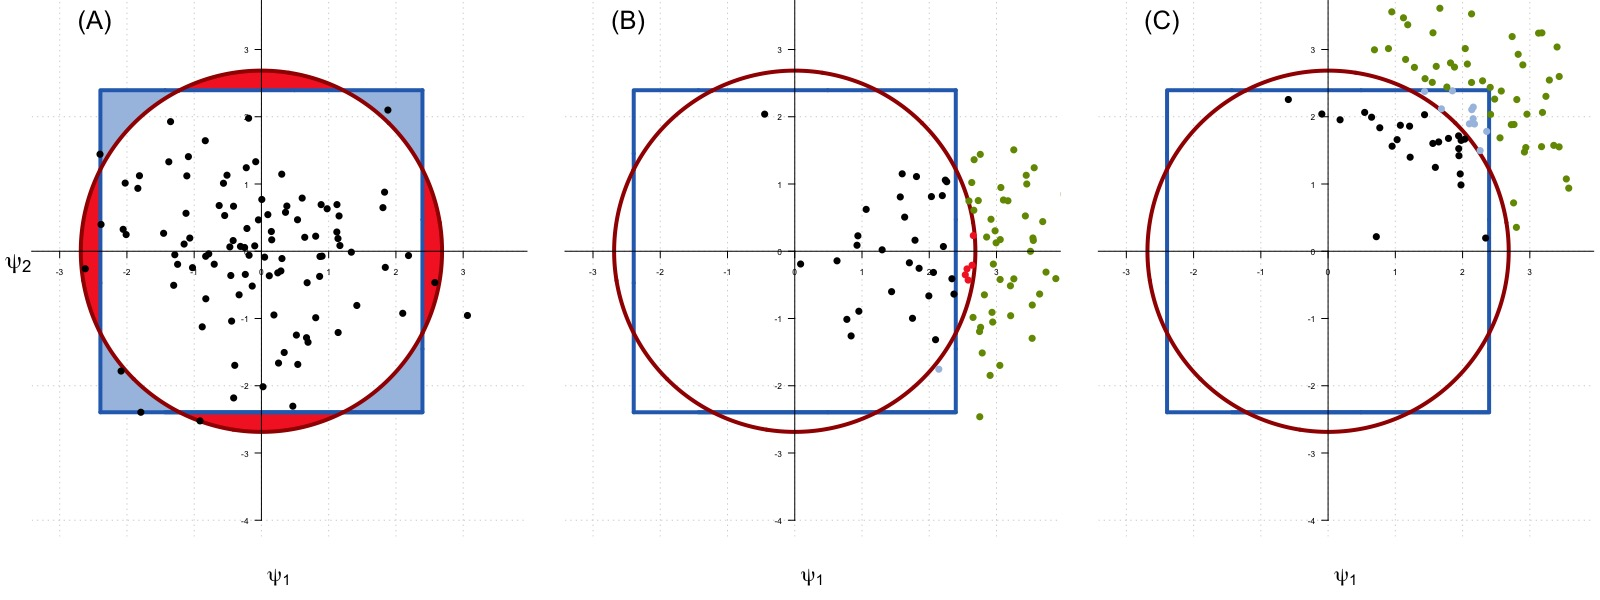
\includegraphics[width = \linewidth]{figure_code/new_pwr_cmpr.jpeg}
	\caption{Plots of 100 observations from a limiting distribution of a hypothetical vector of parameter estimators in $\mathbb{R}^2$ (A) under the null, (B) under an alternative with $\psi_1 = 0, \psi_2 \neq 0$, and (C) under an alternative with $\psi_1, \psi_2 \neq 0$. The 95\% quantiles for the data based on the max (blue) and $\ell_2$ (red) norms under the null are given in all three panels. If a test statistic fell within the blue regions the test would fail to reject $H_0$ if the $\ell_\infty$ norm was used, but would reject $H_0$ if the $\ell_2$ norm was used.  The converse is true for the red regions.  Depending on the alternative, the $\ell_\infty$ norm (B) or the $\ell_2$ norm(C) will achieve higher power.}
	\label{fig:figure1}
\end{figure}

So far, we have outlined a method to construct a test of $H_0$, but it is easy to imagine other tests defined using different norms. With so many potential tests to consider, it is natural to wonder if tests based on different norms have different power, and if so how can someone select the norm with optimal power. To explore the first question, consider a simple example comparing the test described in equation \eqref{eqn:simp_test} with a test that is identical except it uses the maximum absolute deviation or $\ell_\infty$ norm (maximum absolute value) in place the $\ell_2$ norm.  Letting $\boldsymbol{x} = (x_1, \dots, x_d)$ then $\ell_\infty(\boldsymbol{x}) = \max\left\{|x_1|, \dots, |x_d|\right\}$.  Figure \ref{fig:figure1}, panel (A) illustrates these two tests in $\mathbb{R}^2$. One hundred draws are taken from $\nrvs$, a surrogate for the estimated limiting distribution of $\tst$. The random variable $\nrvs$ is a bivariate normal distribution with mean zero and identity covariance matrix. All observations in panel (A) except the five with the largest $\ell_2$ norm are contained within the red circle. The blue square contains all observations in panel (A) except the five with the largest $\ell_\infty$ norm.  The circle and square represent the acceptance regions of tests using empirical estimates of the $95^{\text{th}}$ percentile of $\ell_2(\nrvs)$ and $\ell_\infty(\nrvs)$ respectively corresponding to $r_\alpha(P)$ from \eqref{eqn:ra}.  The same square and circle are redrawn in panels (B) and (C) to illustrate the performance of the test under two alternatives. Observations that fall within the blue shaded region would result in a rejected null hypothesis if the $\ell_2$ norm was used to define the test, but not if the $\ell_\infty$ norm was used. The converse is true of the red shaded region. Panel B shows draws from an alternative in which $\psi_2 \ne 0$ and $\psi_1 = 0$, and panel C shows draws from an alternative in which $\psi_1$ and $\psi_2 \neq 0$. 

While both acceptance regions are created to achieve asymptotic type one error control, depending on the alternative one test will outperform the other. Panel $B$ shows an alternative in which only $\psi_2$ is non-zero.  Because the max norm only considers the largest coordinate, shifting each observation in only a single direction will have larger impact on the max norm of the observations compared to the $\ell_2$ norm.  This trend is shown by the numerous red observations outside of the blue box (equivalent to rejecting $H_0$) and inside the red circle (equivalent to failing to reject $H_0$). In contrast, there is only a single observation that is outside the red circle, and inside the blue box. The converse trend is shown in panel $C$. Here, the $\ell_2$ norm performs better, because it takes into account both coordinates of the shift whereas the $\ell_\infty$ norm can only take into account one of these coordinate shift. 

The efficiency that can be gained from using the correct norm can be quite large, especially in high dimension settings.  Work done by \citep{pinelis_schur2-concavity_2014} states that even for dimensions as small as $3$ the gains in asymptotic efficiency for selecting the correct norm can become arbitrarily large between two potential norms \textcolor{blue}{Review this}.  

% For every distribution $\distv$ with support contained in $\mathbb{R}^d$, let $\Gamma_{\distv}$ be a function mapping from  $\mathbb{R}^d$ to $\mathbb{R}$. The distribution of $\Gamma_\distv(\rvv)$ (where $\rvv \sim \distv$) can be compared to $\Gamma_\distv(\sqrt{n}\hat{\boldsymbol{\psi}})$ to obtain p-values and define a test.  
% \textcolor{blue}{I see $\Gamma_{\distv}$ being an $\mathbb{R}^d$ to $\mathbb{R}$ function. I don't see $\Gamma_Q(x)$ being a function? I also don't understand how this maps ``from a ... distribution'' to anywhere? Do you mean: ``For any distribution $Q$ with support contained in $\mathbb{R}^d$, let $\Gamma_Q$ be a function mapping from $\mathbb{R}^d$ to $\mathbb{R}$''?}
% \textcolor{blue}{What is $\tilde\rvv \overset{d}{=} \rvv$ telling us? Don't we already know that the probabilities over both of these quantities are indexed by $Q$? Also, why use different notation at all? Why not just $\rvv^*$ for both? Here because $c_{0.8}$ is not random so this is distinction does not need to be made.}
% In this scenario, the test can be carried out by comparing our test statistic, $\Gamma_\vmat(\sqrt{n}\hat{\boldsymbol{\psi}}, \|\cdot\|)$ to $\Gamma_\vmat(\rvv, \|\cdot\|).$

% This test statistic was then compared to the estimated limiting distribution of the test statistic under the null.  The key components of this test were to create a real valued summary of the observed test statistic, and compare this test statistic to draws of the test statistic under the null.  In the previous example, the test statistic was the quantile of the $\ell_2$ norm of our vector of parameter estimates.  We already know the distribution of this statistic is uniform from zero to one under the null, so calculating the p-value is trivial.

% However, we could consider other test statistics.  One example would be the estimated power of an observation is from the $80\%$ quantile of the limiting distribution under the null.  Here, while smaller values indicate more evidence against the null, the distribution of this test statistic is not as straightforward.  While more difficult, the distribution of this test statistic can be be estimated using a bootstrap.  We can take a single observation from our estimated limiting distribution of $\sqrt{n}\hat{\psi}$ and then find its multiplicative distance from the $80\%$ quantile under the $\ell_2$ norm.  This can be done many times to create a limiting distribution of our test statistic.  A p-value can then be obtained by comparing the test statistic to the bootstrapped test statistics.	 

\subsection{Adaptive selection of a norm}
In the previous section we showed that a test can be defined with a summarizing function and norm. However, the choice of norm can influence the power of the test. In many scenarios it will not be clear a priori which test will have maximal power because the power of each test depends on the unknown value of the true alternative. The procedure proposed in this section data adaptively selects a norm to attain some of the power improvements that can be attained from selecting the best norm without needing to specify the norm a priori. It will be shown via simulation that this procedure can achieve greater power than a test with a fixed norm.  It will also be shown with  both theory and simulation that this adaptive procedure maintains type 1 error control for large sample sizes.  

% The test defined in \eqref{eqn:simp_test} is a function of three objects; the chosen norm, $\sqrt{n}\hat{\boldsymbol{\psi}}$, and the limiting distribution of  $\hat{t} = \sqrt{n}\hat{\boldsymbol{\psi}}$. Note that the limiting distribution of $\hat{t}$ under the null will always be a multivariate normal with mean zero with some covariance $\Sigma$. Thus potential tests can be defined using the finite dimensional $\Sigma$ matrix rather than the infinite dimension distribution $Q(P)$.

To define norm data adaptive selection rules it will be important to measure the performance of each test. These measures will be referred to as performance metrics and will be denoted by $\Gamma$. While these metrics can be quite general, they should provide an ordering in which better performance results in a more extreme measure of performance. These metrics should provide reasonable comparisons across norms.  For example if one were to use the $\ell_p$ of the test statistic as the performance metric, the first criteria would be satisfied because for most definitions of ``large'' as $x$ grows large, so does $\|x\|_p$.  However, the second criateria is not satisfied because $\ell_1(x) \geq \ell_2(x) \geq \dots \geq \max(x)$, it does not satisfy the second criteria. 

In order to achieve both criteria mentioned previously, the performance metrics considered in this paper will be functions of both the test statistic $\tst$ and the limiting distribution of the test statistic $\rvt$ under the null. The limiting distributions will allow us to understand how extreme $\tst$ is relative to what we would see under the null which allows us to make comparisons across norms.

As an asside, note that the limiting distribution of $\tst$ under the null will always be a multivariate normal with mean zero with some covariance $\Sigma$. Thus potential tests can be functions of the finite dimensional $\Sigma$ matrix rather than the infinite dimension distribution $Q(P)$. To maintain consistency throughout this paper performance metrics will have the added condition that they become smaller as performance improves. This condition is discussed more in section \ref{sec:test_cnsty}. If a candidate performance metric becomes large as $\tst$ grows large, the reciprocal of this performance metric can be used. Performance metrics can be thought of analogously to the p-value of a test in which a non-adaptive version of the test was used.

% While all tests will reject as the test statistic becomes larger, if the measure of performance was the norm $\hat{t}$ then the optimal norm would always be the $\ell_1$ norm.  To achive this goal, we will consider other mappings from $\mathbb{R}$ into $\mathbb{R}$ that are comparable across norms.
% Consider a general function $\Gammaf$, of a vector in $\mathbb{R}^d$ (corresponding to $\tst$). There is a requirement that $\Gammaf(x)$ should get smaller as $x$ moves away from the null, $\Gammaf$ can be quite general.
The first performance metric we consider is the acceptance rate of the test defined in  \eqref{eqn:simp_test} if $\psi = \tst$: 
\begin{align}
	\Gamma(x, \Sigma) &= Pr_\distv(\|\rvt + x\| \leq c_{0.8})  \text{ where }  c_{0.8} \equiv \min_{c}\{c : Pr(\|\rvt\| < c) \geq 0.8 \} \text{ and } \rvt \sim N(0, \Sigma). \label{gamma:pow}
\end{align}

We can define a test using $\Gamma$: 
\begin{align*}
	\text{reject } H_0 \text{ if } \Gamma(\tst, \Sigma) \leq c_{1 - \alpha} \text { where } c_{1 - \alpha} = \min_{c}\{c : \text{Pr}(\Gamma(\rvt, \Sigma) \geq c) < \alpha\} \text{ where } \rvt \sim N(\boldsymbol{0}, \Sigma)
\end{align*}
% \textcolor{blue}{I don't understand the end of this sentence}. 
% While the the above test has nice properties (type one error control, consistency), it is not clear how this test will perform compared to other tests with similar properties.

% by defining a $\Gamma$ to those defined earlier, except the optimal norm is selected, and the corresponding summary value of $\Gamma$ with the optimal norm is returned.  For example, if we had $p$ different norms, $\norm_1, \dots, \norm_p$ and some summary function $\Gamma_\vmat(x, \|\cdot\|)$, we would define the adaptive version of $\Gamma$ as
\begin{align*}
	\Gamma^*(x, \Sigma) = \min\left\{\Gamma_{1}(x, \Sigma), \dots, \Gamma_{p}(x, \Sigma)\right\}.
\end{align*}

While this function is more complicated than before, distribution of $\Gamma^*(\rvt, \Sigma)$ can still be compared to $\Gamma^*(\tst, \Sigma)$ to obtain a p-value. Also, while it may be difficult to obtain the exact distribution of $\Gamma^*(\rvt, \Sigma)$, the distribution is a function of $\vmat$, so obtaining good approximations of $\Gamma^*(\rvt, \Sigma)$ is possible by taking many draws from $\rvt$.

% Let $g_1, \dots, g_k$ be a list candidate norms, and let $\boldsymbol{Z}_1, \dots, \boldsymbol{Z}_B$ and $\boldsymbol{V}_1, \dots, \boldsymbol{V}_B$ independent draws from $Q$.  For each of the possible norms, let a p-value be defined using the following quantity:

% \begin{align*}
% s_{p}\left(\sqrt{n}\hat{\boldsymbol{\psi}}, \boldsymbol{Z}_1, \dots, \boldsymbol{Z}_B\right) = \frac{1}{B}\sum_{i=1}^B I\left\{g_p\left(\sqrt{n}\hat{\boldsymbol{\psi}}\right)  \leq g_p(\boldsymbol{Z}_i)\right\}
% \end{align*}

% Using the $c_{p, \alpha}$ defined earlier, it is possible to obtain estimates of power for each norm for any assumed vector of parameters:
% \begin{align*}
% \hat{\omega}_{\alpha, p}(\boldsymbol{h}) = \frac{1}{B} \sum_{i=1}^B I\left\{g_p\left(\boldsymbol{h} + \boldsymbol{V}_i\right) \geq \hat{c}_{\alpha, p}\right\}
% \end{align*}
% The last quantity considered is the multiplicative distance the vector of parameter estimates is from a vector in the same direction which obtains a certain power:
% \begin{align*}
% \hat{r}_{\alpha, p}(a) = \min\left\{r : \hat{\omega}_{\alpha, p}(r \times \sqrt{n}\hat{\boldsymbol{\psi}}) > a\right\}
% \end{align*}
% As described above, there are a multitude of ways to evaluate the performance of the various norms.  Let $f_p(x_1, \dots, x_k)$ be the function that takes the observed data and a norm and returns a measure of the norm's estimated performance given the observed data. $f$ could be $s_p$, $\hat{\omega}_{\alpha, p}$, $\hat{s}_{\alpha, p}$, or some other function.  Let $p^*$ be the index of the ``optimal'' norm.  What is optimal depends on $f$.  If $f$ is the p-value measure $s_p$ then the optimal norm minimizes the $p-value$.  However if instead $f$ is estimated power, then the optimal norm maximizes estimated power.     

% Define the test statistic $\hat{t}$ as 
% \begin{align*}
% \hat{t} = f_{p^*}(\boldsymbol{x}_1, \dots, \boldsymbol{x}_n)
% \end{align*}
% While it is not necessary to do this, the same $f$ used for norm selection will be used to define our test statistic.

\subsection{Obtaining the null distribution}
\label{ssec:obtaining_null}
The described procedure requires knowledge of the limiting distribution of $\rnp$ when $P \in \mathscr{M}_0$.  To obtain an estimate of this limiting distribution, we require that each of the estimators $\rnp_1, \dots, \rnp_d$ of $\boldsymbol{\psi}_1, \dots, \boldsymbol{\psi}_d$ is asymptotically linear.  That is for each $j \in \{1, \dots, d\}$:
\begin{align*}
\hat{\psi}_j = \psi_j + \frac{1}{n}\sum_{i=1}^n D_j(\boldsymbol{x}_i) + o_p(1/\sqrt{n}) \text{ for some function } D_j
\end{align*}

Where the $D_j$ function will be referred to as an influence function. Most standard estimators of association are asymptotically linear and have known influence functions.There also exists a growing body of literature describing asymptotically linear estimators and their corresponding functions \textcolor{blue}{Need citations here}.

% $\sqrt{n}\hat{\boldsymbol{\psi}}$, converges to a normal distribution with an estimable variance covariance matrix when properly centered and normalized.

When there is a fixed number of covariates, the Cramer-Wold device can be used to show that $\sqrt{n}( \hat{\boldsymbol{\psi}}  - \boldsymbol{\psi})$ estimates is asymptotically normal with mean zero, and variance covariance matrix given by $\Sigma = E_{\disto_0}\left[D(\rvo) D(\rvo)^\top \right]$:
% \textcolor{blue}{Note from Alex: do you mean $D(\rvo) D(\rvo)^\top$? This is what you would want if $D(\rvo)$ were a column vector, which would be more standard (similar comment in other places where `$\top$' is used)}
\begin{align*}
    \sqrt{n}\left(\hat{\boldsymbol{\psi}} - \boldsymbol{\psi}\right) \xrightarrow{d} \rvt \sim N\left(0, \Sigma\right)
\end{align*}

Under $H_0$, $\rnp$ converges to $\rvt$, and $\Sigma$ can be consistently estimated using $\widehat{\Sigma} = \frac{1}{n}\sum_{i = 1}^n D(\boldsymbol{x}_i) D(\boldsymbol{x}_i)^\top$.  In practice, a consistent estimator of $\vmat$, $\hat{\vmat}$ will be used in place of $\vmat$ for the calculation of $\tst$. Thus, the test statistic will be $\Gamma(\tst, \hat{\Sigma})$ will be compared to $\Gamma(\hat{\rvt}, \hat{\Sigma})$ where $\hat{\rvt} \sim N\left(0, \hat{\Sigma}\right)$.

\subsection{Using a permutation test for the test statistic}
While the above approach works asymptotically, for small sample sizes there can be greater than $\alpha$ type one error.  To avoid this, a permutation based test can be used in certain settings. 

Letting $\Pi$ be the set of all $n!$ one-to-one functions mapping from $\{1, \dots, n\}$ to $\{1, \dots, n\}$, let  $\pi_1, \dots, \pi_B$ be drawn uniformly from $\Pi$ with replacement. To carry out the permutation test test, $B$ draws are taken from the null distribution where each the $j^{\text{th}}$ draw is the test statistic $\sqrt{n}\hat{\boldsymbol{\psi}}^{\#}_j$ for a permuted data set $(y_{\pi_j(1)}, x_{1, 1}, \dots, x_{1, d}), \dots, (y_{\pi_j(n)}, x_{n, 1}, \dots, x_{n, d})$.  After taking these draws, a p-value can be calculated $B^{-1}\sum_{i = 1}^B I\{\sqrt{n}\hat{\boldsymbol{\psi}} \geq \sqrt{n}\hat{\boldsymbol{\psi}}^{\#}_i\}$ and the corresponding test rejects the null if this $p-$value is less than $\alpha$. 

This approach can only be applied in settings in which the null hypothesis corresponds to all used covariates being jointly independent of the outcome.  For example if the parameter of interest is a conditional association measure as is the case in the second and third examples, this procedure will not work.  


\section{Theoretical Results}
\label{sec:theorems}
While we try to keep theoretical results as general as possible, in order to establish consistency and  non-trivial local ubiasedness of the testing procedure we place restrictions on the norms and performance metrics. 

\subsection*{Performance metric and norms considered}
In the examples considered in this article two performance metrics are considered.  The first is the estimated acceptance rate performance metric as described in equation \eqref{gamma:pow}.  The other performance metric considered is the multiplicative distance $\tst$  performance metric defined by:

\begin{align}
	\Gamma(t, \Sigma) = \text{min}\left\{s : \text{Pr}(\|Z + st\|_p \geq c_\alpha) \geq 0.8 \right\} \label{eqn:mult_dist_gam}
\end{align}

Both performance metrics are considered to provide multiple examples of viable performance metrics and because each has its own advantages and disadvantages.  The estimated acceptance rate performance metric has the advantage of being intuitively simple and relatively simple to calculate.  However this metric also is bounded between zero and one which has the potential to cause issues when calculating the limiting distribution if most of the mass of $\Gamma(Y, \Sigma)$ is concentrated near 1.  The multiplicative distance performance metric does not face this constraint, but is more difficult to understand intuitively.  Additionally this metric is more computationally costly, and the $0.8$ used is somewhat arbitrary and it is not clear what effect changing this value would have on the power of tests based on this metric (we hope it has little to no effect).

For both metrics, two sets of norms are considered for the adaptive test.  Letting $\boldsymbol{x} = \left(x_1, \dots, x_d\right)$ the $\ell_p$ norm is defined by

\begin{align*}
 \ell_p(\boldsymbol{x}) = \sqrt[p]{\sum_{i = 1}^d |x_i|^p }
\end{align*}

The second set of norms referred to as the sum of squares norm is a function mapping from $\mathbb{R}^d$ to $\mathbb{R}$ defined by 
\begin{align*}
	\|\boldsymbol{x}\|_k = \sum_{i = 1}^k x_{(d - i + 1)} 
\end{align*}
where $x_{(1)}, \dots, x_{(d)}$ are the order statistics of $x_1, \dots, x_d$. When adaptive versions of either performance metric are used in practice one must specify which norms to select over.  In this work the possible indices ($p$'s) for the $\ell_p$ norm are $1, 2, 4, 6,$ and $\infty$ and the possible indices for the sum of squares norm are the six evenly spaced values between $1$ and $d$ (the dimension of $x$).  If any of these values are not whole numbers they are rounded to the nearest whole number.  

Lemmas \ref{lemma:est_accept} and \ref{lemma:mult_dist_gam} show that the estimated acceptance rate and multiplicative distance performance metrics satisfy these restrictions respectively.  

\subsection{Consistency under fixed Alternatives}

\label{sec:test_cnsty}

Consider the following conditions on the performance metric $\Gamma : \mathbb{R}^d \otimes \mathbb{R}^{d \times d} \mapsto \mathbb{R}$:

\begin{enumerate}
	\item The performance metric $\Gamma$ is continuous and is non-negative
	\item $\pr\left(\Gamma(Z, \Sigma) = 0\right) = 0$ where $Z \sim N(0, \Sigma)$
	\item $E\left[\left|\Gamma^*_{\hat{\Sigma}}(\sqrt{n}\hat{\boldsymbol{\psi}})\right| \right] \rightarrow 0$ for all fixed $P \not \in \mathcal{M}_0$, all consistent estimators $\hat{\boldsymbol{\psi}}$ of $\boldsymbol{\psi}$ and all consistent estimators $\hat{\Sigma}$ of $\Sigma$.
	\setcounter{conditions}{\value{enumi}}
\end{enumerate} 

\begin{theorem}
\label{thm:cnst}
If $\hat{\boldsymbol{\psi}}$ is a consistent estimator of $\psi$, $\hat{\Sigma}$ is a consistent estimator of $\Sigma$, and $\Gamma$ satisfies conditions 1 - 3 then the test defined by
\begin{align*}
	\text{reject } H_0 \text{ if } \Gamma^*(\sqrt{n}\hat{\boldsymbol{\psi}}, \hat{\vmat}) \leq F^{-1}_{\Gamma^*(\hat{\rvt}, \hat{\vmat})}(\alpha)
\end{align*}
is consistent.  
\end{theorem}

\subsection*{Local Unbiasedness}
Consider a sequence of local alternatives $P_n$ in which the value of $\Psi(P_n) = \psi_n = \underline{h}/\sqrt{n}$ shrinks towards zero as $n$ grows.  We wish to show that our test is non-trivially locally unbiased, that is for large $n$:
\begin{align*}
	Pr_{\disto}\left(\gamestp \leq F^{-1}_{\gamestz}(\alpha)\right) > \alpha 
\end{align*}
To achieve this, we fist assume our estimator $\rnp$ is consistent and regular at $\boldsymbol{\psi}$. The estimator $\hat{\boldsymbol{\psi}}$ is regular if and only if for every sequence $\psi_n$ with $\sqrt{n} (\psi_n - \psi) \to \underline{h}$, the sequence $\sqrt{n}(\hat{\psi} - \psi_n) \xrightarrow{P_{\psi_n}} Z$, where $Z$ can be different for different $\psi$, but not for different $t$. Two additional conditions on $\Gamma$ are sufficient to have tests based on $\Gamma$ be locally unbiasedness.

\begin{enumerate}
	\setcounter{enumi}{\value{conditions}}
	\item $\Gamma$ is unimodal for every $\Sigma$ (for every $k$, the set $\{x : \Gamma(x, \Sigma) \geq k\}$ is convex).
	\item $\Gamma$ is centrally symmetric for every $\Sigma$, $(\Gamma(-x, \Sigma) = \Gamma(x, \Sigma))$.
\end{enumerate}

\begin{theorem}
	\label{thm:unbiased_locl_alt}
Let $P_{n}$ be a sequence of local alternatives under which the value of $\Psi(P_n)$ is $\underline{h}/\sqrt{n}$, and let $\nrvs \sim N\left(\boldsymbol{0}, \Sigma\right)$ and  $\hat{Y}_{\Sigma} \sim N\left(\boldsymbol{0}, \hat{\Sigma}\right)$.  If $\Gamma$ satisfies conditions 1, 2, 4, and 5, the estimator $\hat{\Sigma}$ of $\Sigma$ is consistent, and the estimator $\hat{\psi}$ of $\psi$ is regular at $\boldsymbol{\psi}$. Then the test defined by 
\begin{align*}
	\text{ reject } H_0 \text{ if } \gamestp \leq F^{-1}_{\gamestz}(\alpha)
\end{align*}
has power greater than $\alpha$ under $P_n$.
\end{theorem}

\section{Simulation Study}
\label{sec:sim_stdy}

\subsection{Correlation}

% In the first set of experiments, we compare our method to both a Bonferroni based method and a tailor made method.  The Bonferroni based method computes a p-value for each covariate using a marginal linear regression.  If any p-value is smaller than the Bonferroni adjusted cutoff value, the null hypothesis is rejected. The method outlined by \citep{zhang_comment_2015} is similar to our method, but uses a parametric estimate of the correlation instead of using an influence function based estimator.  Four versions of our test are displayed in these plots. Our test that uses the $\ell_2$ norm, our test that uses the $\ell_\infty$ or max norm, and our test that selects over five possible $\ell_p$ norms.  The last version of our test selecs over many different versions of the following norm : $\|x\|_k = \sum_{i = 1}^k x_{(i)}^2$ where $x^2_{(i)}$ are the ordered statistics of $x^2$.

% In each setting, each test is run 1000 times.  The proportion of tests that reject the null is plotted for each simulation setting and for each test.  

\begin{figure}[]
	\centering
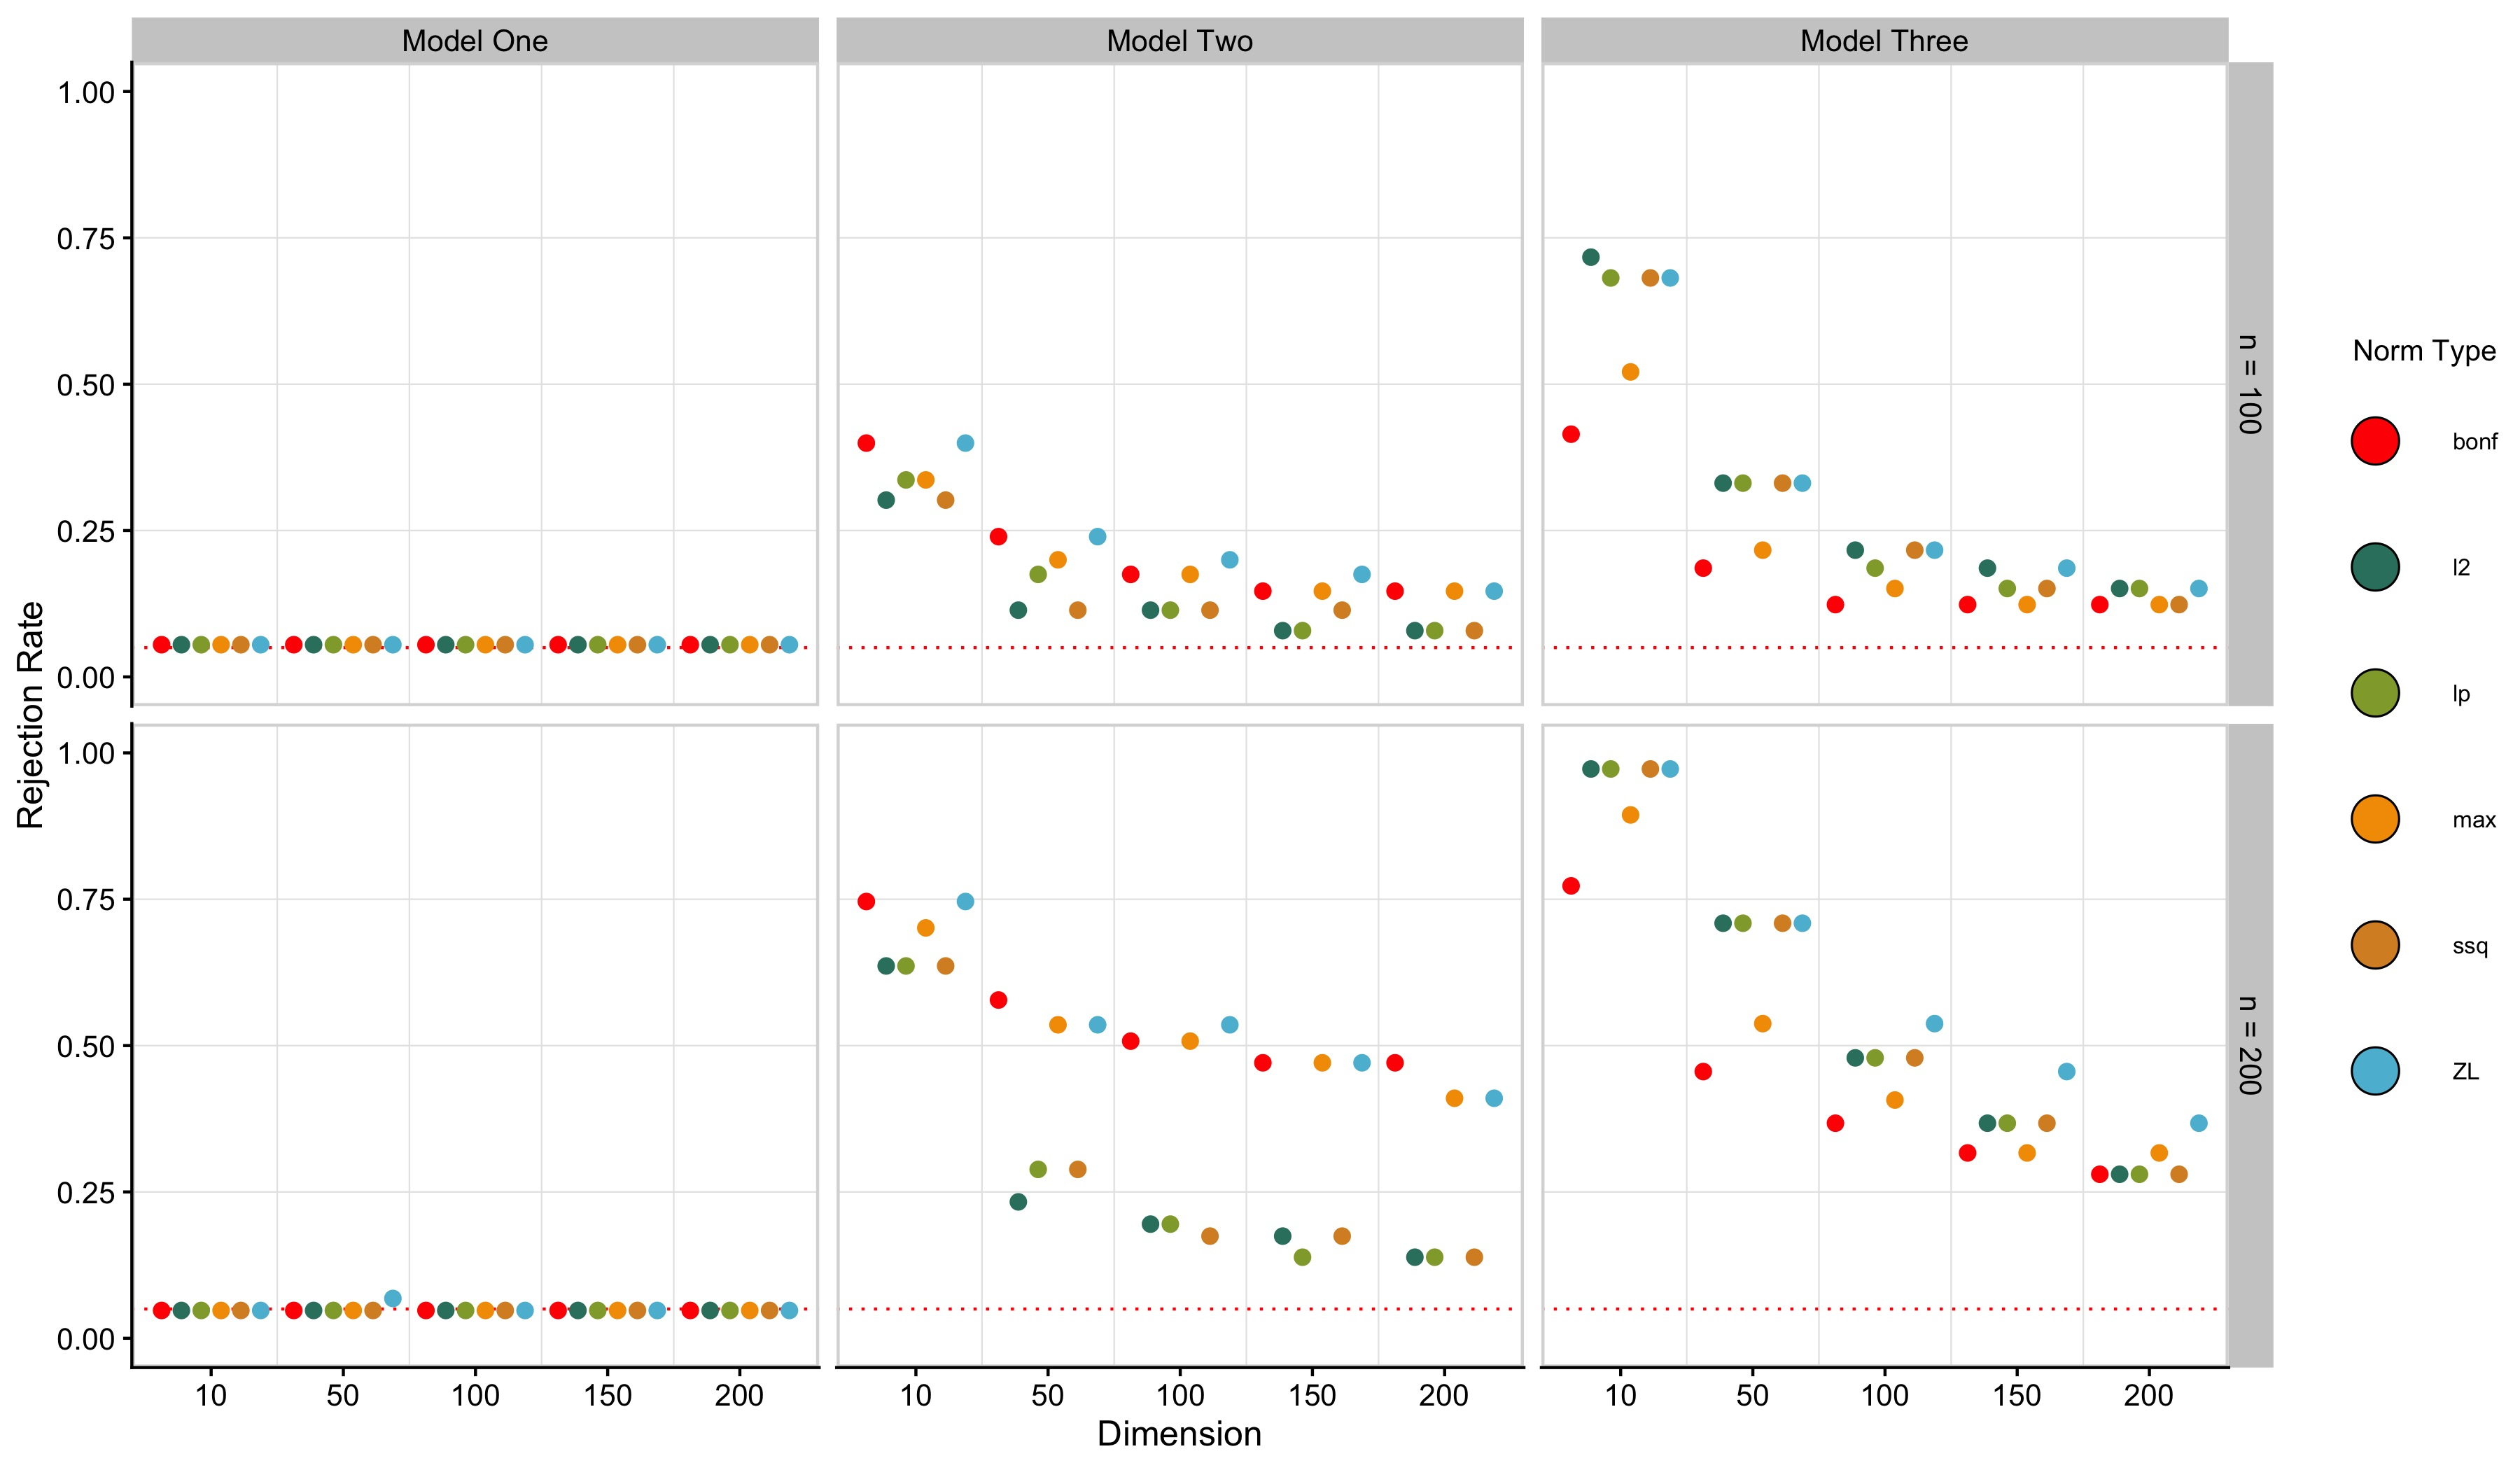
\includegraphics[width = \linewidth]{uncor.jpg}
	\caption{Display of simulations for vector of covariates in this setting will be generated from a normal distribution with mean zero and a variance covariance of $\Sigma$ with $\Sigma_{ij}$ equal to $0$ when $i \neq j$ and equal to 1 when $i = j$. Three different models for the outcome of interest ($Y$) will are considered. Letting $\varepsilon \sim N(0, 1)$ and be independent of $W$, in the first model $Y = \varepsilon$, in the second $Y = W_1 / 4$, and in the third $Y = \sum_{k = 1}^{10} \beta_k W_k + \varepsilon$ where $\beta_k = 0.15$ for $k = \{1, \dots, 5\}$, and $\beta_k = -0.1$ for $k = \{6 \dots 10\}$. Sample sizes of $100$ and $200$, dimensions of $10$, $50$, $100$, $150$, and $200$ are considered.}
	\label{fig:uncor}
\end{figure}

\begin{figure}[]
	\centering
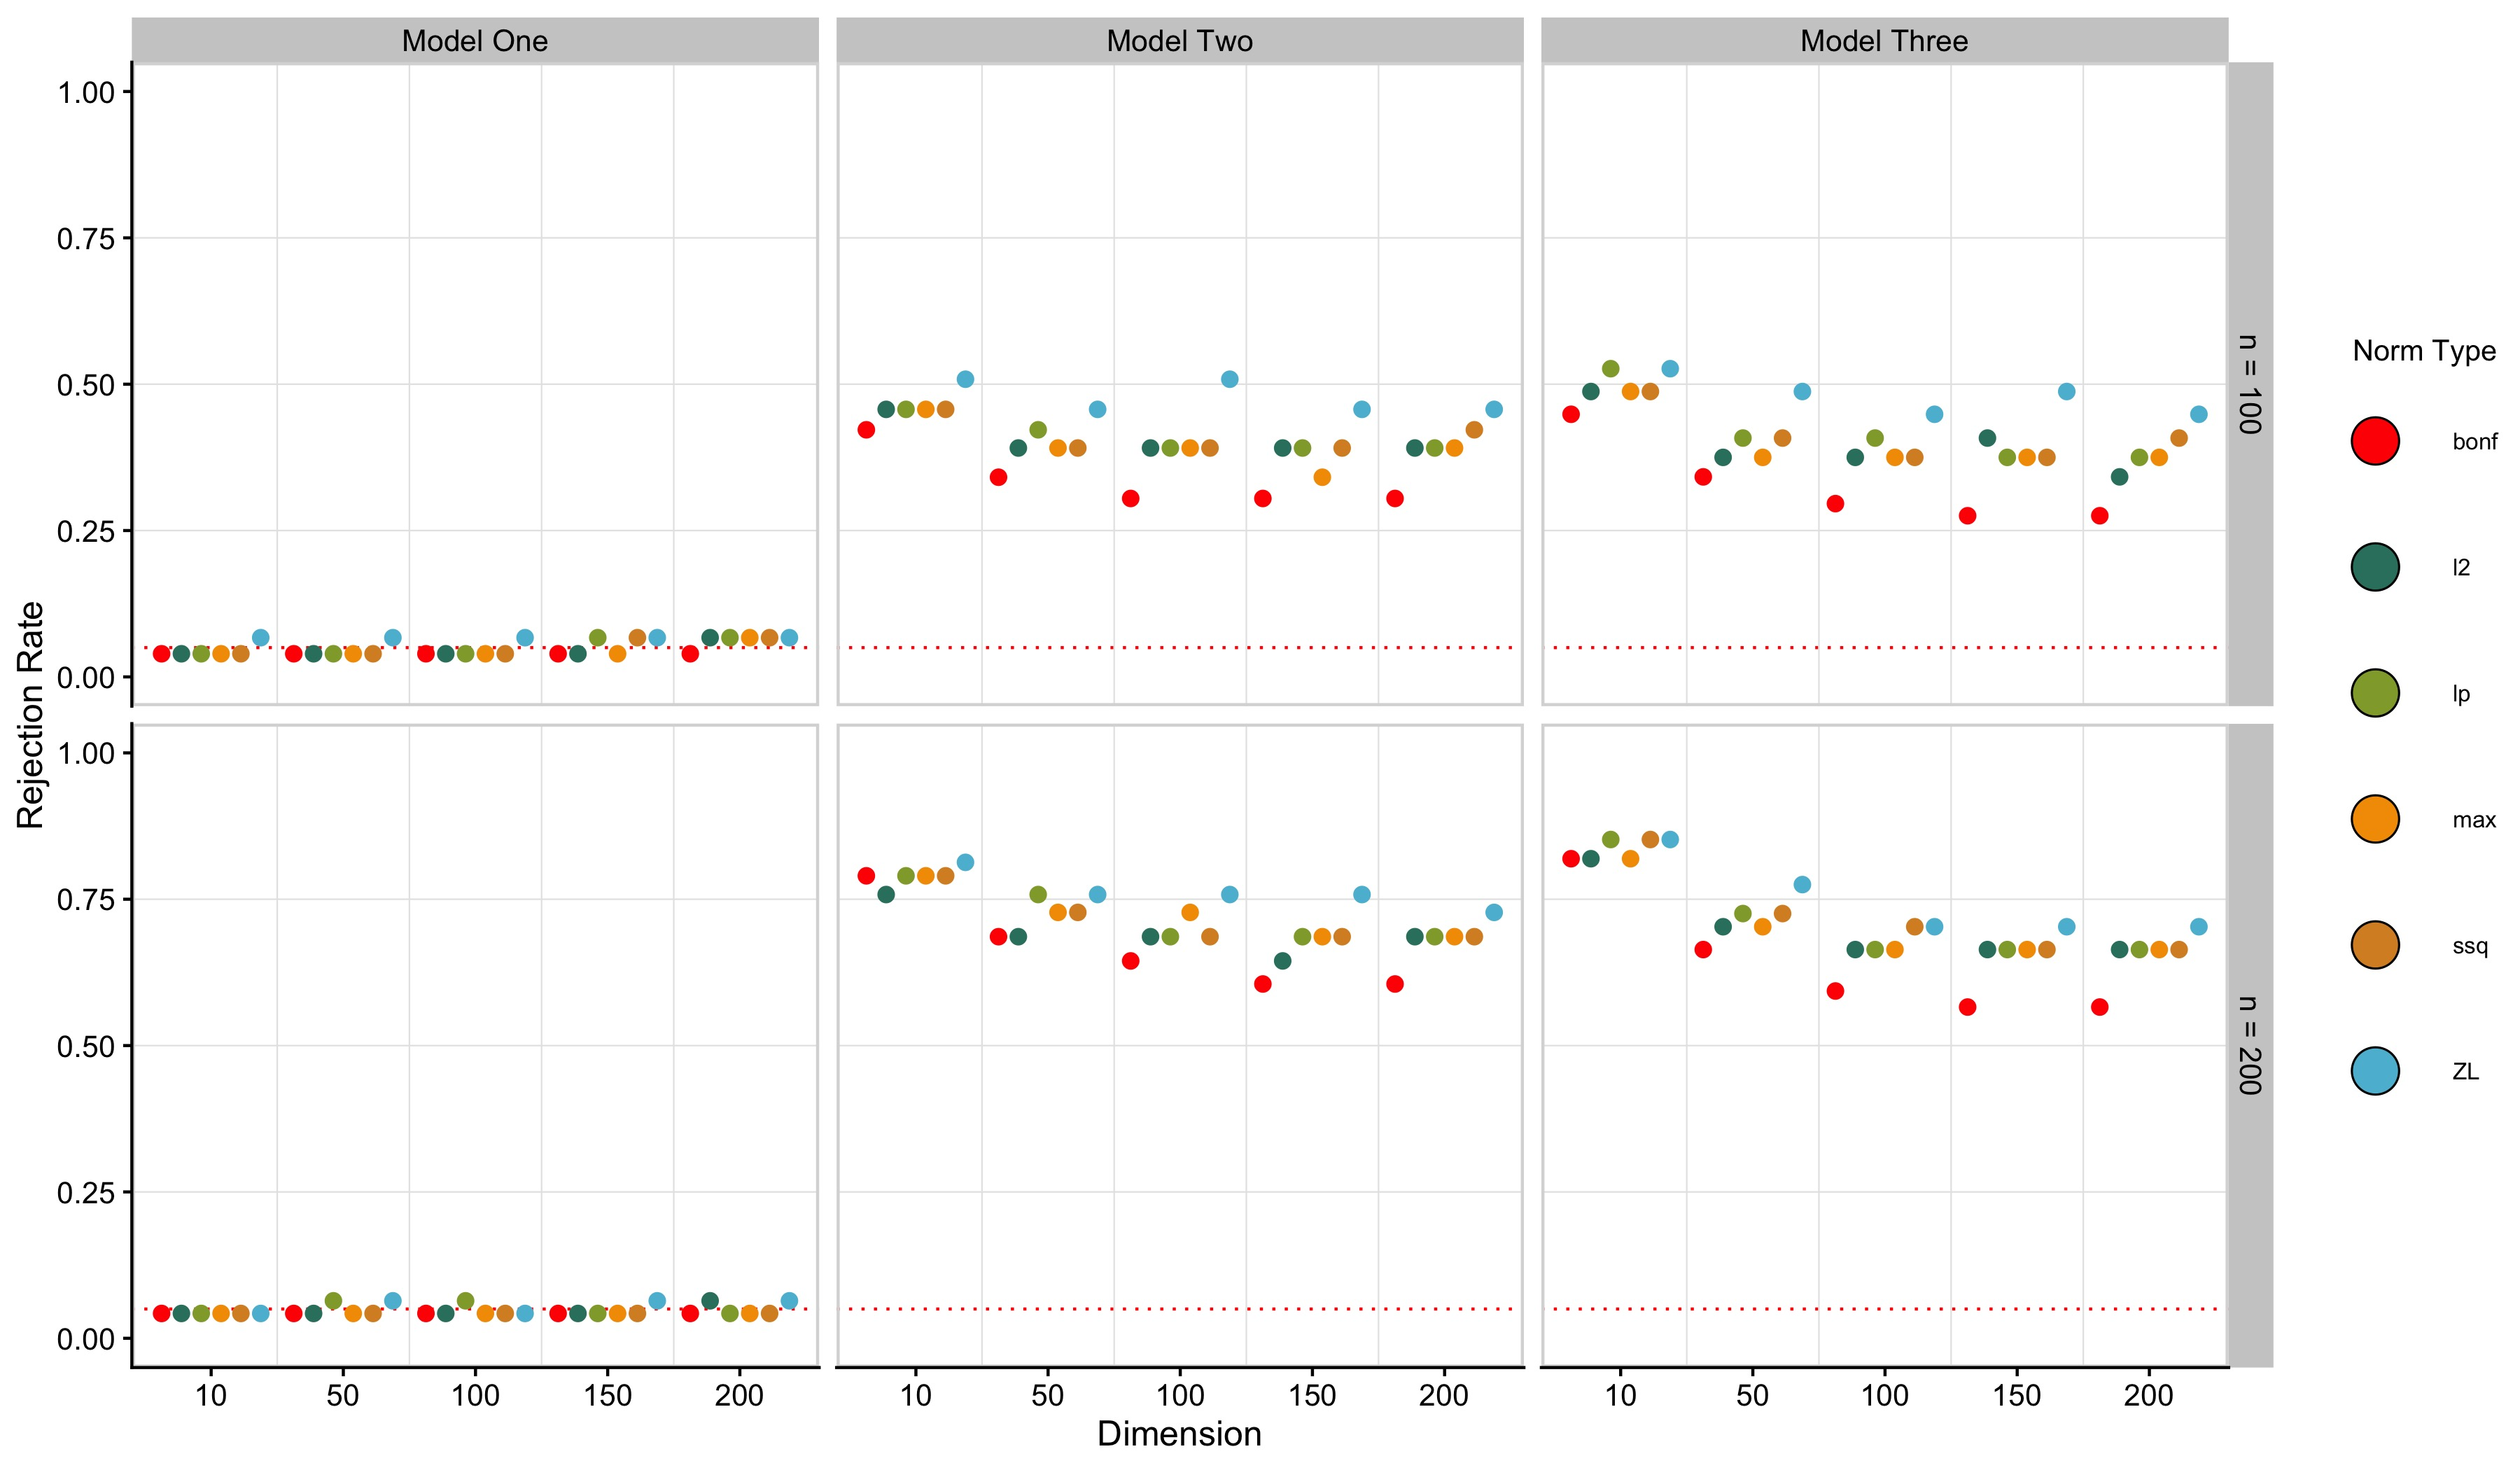
\includegraphics[width = \linewidth]{some_core.jpg}
	\caption{The same simulation settings as those used in Figure \ref{fig:uncor}, but $\Sigma_{ij} = 0.5$ for $i \neq j$.}
	\label{fig:somecor}
\end{figure}	

\begin{figure}[]
	\centering
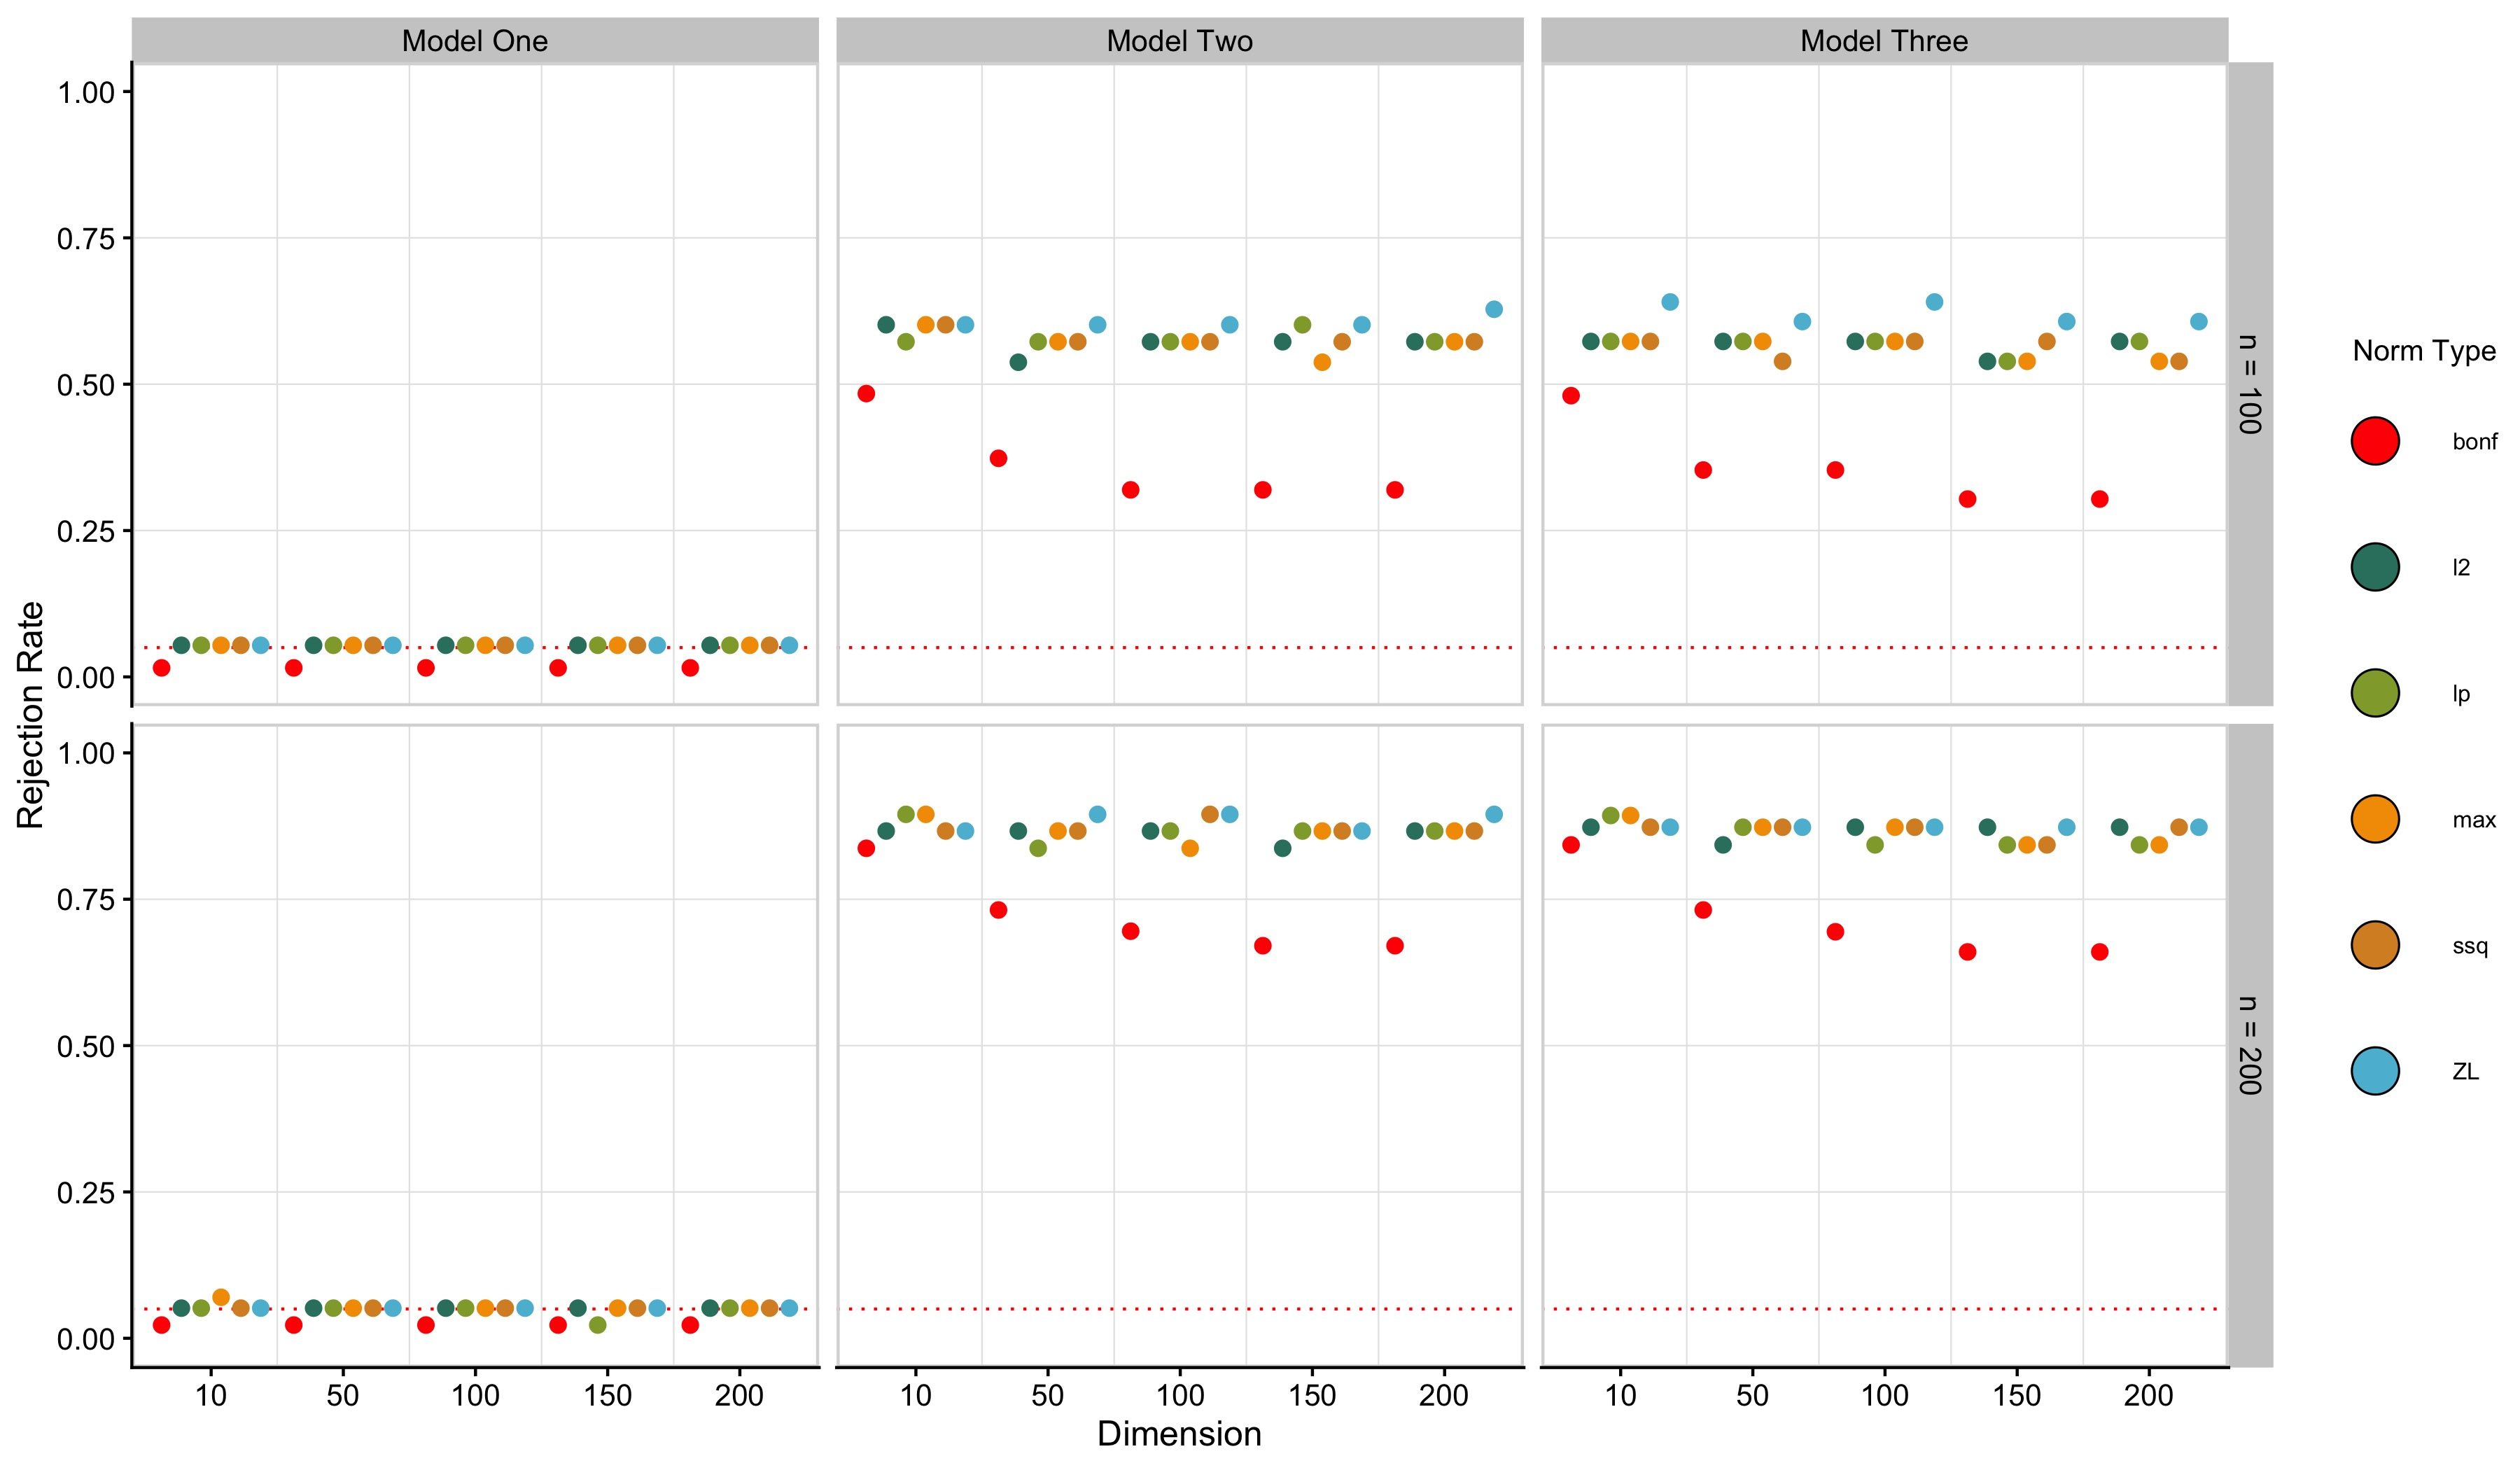
\includegraphics[width = \linewidth]{lots_cor.jpg}
	\caption{The same simulation settings as those used in Figure \ref{fig:uncor}, but $\Sigma_{ij} = 0.8$ for $i \neq j$.}
	\label{fig:lotscor}
\end{figure}

% We find that our procedure uses obtains relatively good power across a variety of settings.  While in certain settings our test is beaten by that of Zhang and Laber, this is to be expected because their procedure is tailor made for the setting in which there is normal data that follows a linear model. We also find that the adaptive version o the test consitently outperforms the Bonferroni based method in all settings except those in which there is no between-covariate correlation.

In figures (\ref{fig:uncor}, \ref{fig:somecor}, \ref{fig:lotscor}), the rejection rates of six different tests are shown for a wide variety of settings. Each test has the null hypothesis that $\psi_1, \dots, \psi_d = 0$ where $\psi_i = \Psi_i(P)$ is the correlation between the outcome $Y$, and the $j^\text{th}$ covariate $W_j$. A description of the data generating mechanism can be found in section \ref{sec:Working Examples}.  Red dots indicate a bonferroni adjusted marginal test for the estimated correlation between each covariate and the outcome. Light blue dots indicate the performance of the test proposed by [Zhang and Laber]. The other colors correspond to different variants of our test. Dark green and yellow dots indicate the performance of our test using only the $\ell_2$ or maximum absolute value norm respectively.  The light green dots indicate the performance of our test when it adaptively select one of the $\ell_p$ norms. Brown dots indicate our tests performance when the test adaptively selects over various sum of squares norms. The dotted red line in each plot indicates the $0.05$ rejection rate that should be observed when $H_0$ holds.  

Because $H_0$ is true for model one, we expect the rejection rates for this model to be $0.05$.  Figures \ref{fig:uncor}, \ref{fig:somecor}, and \ref{fig:lotscor} show these rates are achieved by every testing procedure except the bonferroni based test which is somewhat conservative.  For the other two models, $H_0$ does not hold so these plots compare the powers between the different testing procedures.  The bonferroni based test has the lowest power in all of the considered settings and for larger numbers of covariates this differences is larger. All other tests have similar power in most settings, with the test proposed by [Zhang and Laber] performing slightly better in most settings where a difference exists.  All tests perform better for larger sample sizes, but tend to perform similarly for varying dimension and generating model.

One setting in which the adaptive test performs poorly is in settings in which a single covariate is correlated with the outcome of interest and no covariates are correlated as seen for model 2 in figure \ref{fig:uncor}. This behavior could be due to the parameter estimates inability to be sparse even in settings when sparsity occurs.  The many small errors in the parameter estimate across many covariates leads to a preference for the $\ell_2$ norm that obtains an overly optimistic estimate of power due to the accumulation of many small effects across all the covariates.

% A wide variety of simulation settings are considered in this section to show the breath of settings in which the adaptive test can be used.  The first setting considers independent draws from a random vector with mean zero and variance-covariance matrix $\Sigma$.  The measure of association between $Y$ and each covariate will be $\text{Cov}(Y, W_{j})/\text{Var}(W_j)$.  The dimension of the vector, denoted $d$ takes values $10, 50$, and $200$.  The number of correlated covariates will be zero, one, or $0.1, 0.2$, or $0.6$ of all the correlated covariates.  The correlation between each of the covariates will be either $0$ or $0.5$.  The sample sizes considered are $100$ and $500$.   

\subsection*{Two Phase Sampling Risk Ratio}
The for the second example was carried out after deriving the influence of the parameter given in equation \ref{eqn:DE2param}. Marginal expectations were estimated using either an elastic net \citep{simon_blockwise_2013,tibshirani_strong_2012,friedman_regularization_2010, tibshirani_strong_2012} or a superlearner \citep{polley_super_2010}.

Figure \ref{fig:dat_examp_2} shows the rejection rates of four different tests across the settings described in section \ref{sec:data_app}. Each test has the null hypothesis that $\psi_1, \dots, \psi_d = 0$ where $\psi_i = \Psi_i(P)$ is the risk ratio that $Y = 1$ comparing two observations which differ by a unit in the covariate $W_j$. Data are generated using three  different settings.  In the first setting no covariates are directly associated with the outcome ($H_0$ holds), in the second setting a single covariate has a strong, direct association with the outcome ($H_0$ does not hold), and in the third setting ten covariates are directly associated with the outcome ($H_0$ does not hold). Each color of dots represents a different version of our test. Red and light green dots indicate the performance of our test using only the $\ell_2$ or maximum absolute value norm respectively.  Dark green dots indicate the performance of our test when it adaptively select one of the $\ell_p$ norms. Yellow dots indicate our tests performance when the test adaptively selects over various sum of squares norms. The dotted red line in each plot indicates the $0.05$ rejection rate that should be observed when $H_0$ holds. 

% Here, we would expect that the $\ell_2$ norm would perform poorly in the model 2 setting while performing well in the model 3 setting, and that the max norm would perform poorly in the model three setting while performing well in the model two setting.  However, we see the opposite behavior.  Additionally, we find that our adaptive test performs well consistently across all alternatives. 
\begin{figure}[H]
	\centering
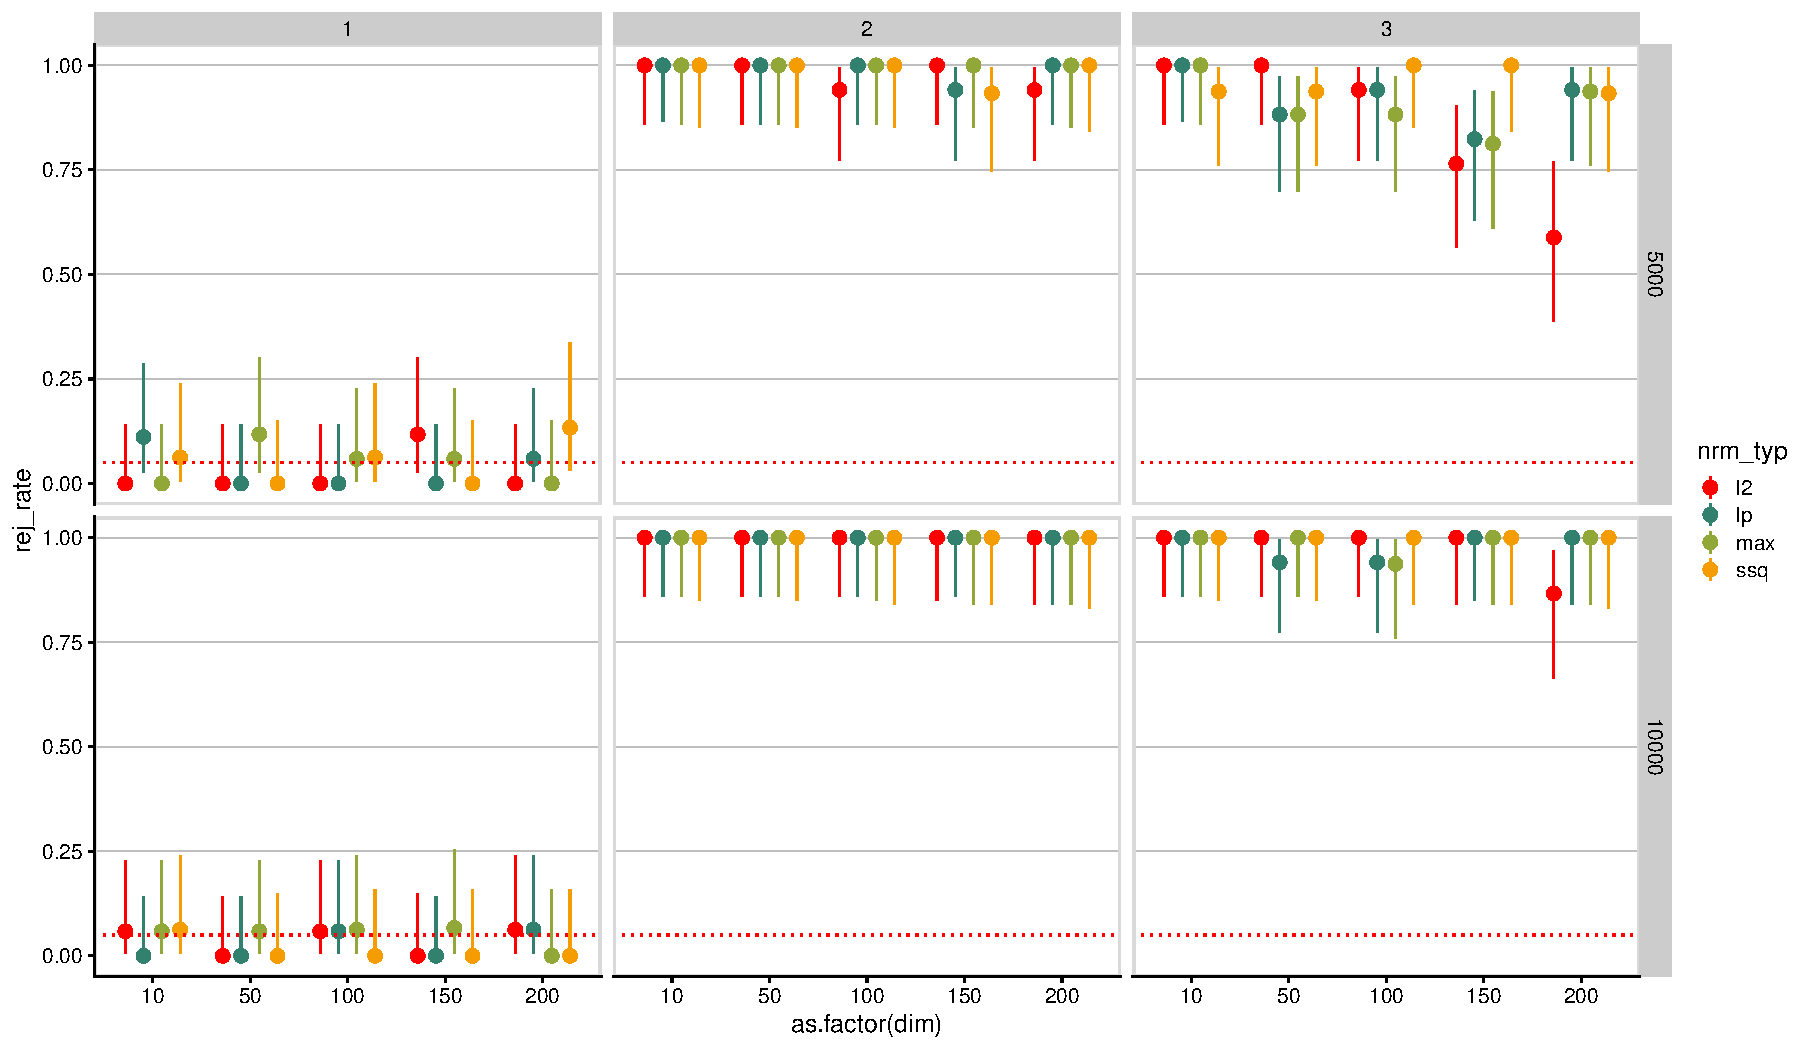
\includegraphics[width = \linewidth]{mag_w_unc_de2.pdf}
\label{fig:dat_examp_2}
	\caption{Rejection rates across three different data generating mechanisms. Here we are using the multiplicative distance our test statistic is from obtaining 80\% power as our measure of performance.}
	\label{fig:magnitude}
\end{figure}

\subsection*{Marginal Structural Model}
Testing for this example was carried out using code from the ltmle package \citep{lendle_ltmle_2017} to estimate the influence function of our parameter.  Using this estimate of the influence function, a parametric bootstrap was used to estimate the limiting distribution of our test statistic.  The multiplicative distance performance metric was used for these simulations. Data are generated using three  different settings.  In the first setting no covariates modifies the treatment effect ($H_0$ holds), in the second setting a single covariate modifies the treatment effect ($H_0$ does not hold), and in the third setting ten covariates modify the treatment($H_0$ does not hold). Each color of dots represents a different version of our test. Red and light green dots indicate the performance of our test using only the $\ell_2$ or maximum absolute value norm respectively.  Dark green dots indicate the performance of our test when it adaptively select one of the $\ell_p$ norms. Yellow dots indicate our tests performance when the test adaptively selects over various sum of squares norms. The dotted red line in each plot indicates the $0.05$ rejection rate that should be observed when $H_0$ holds. 

\begin{figure}[H]
	\centering
	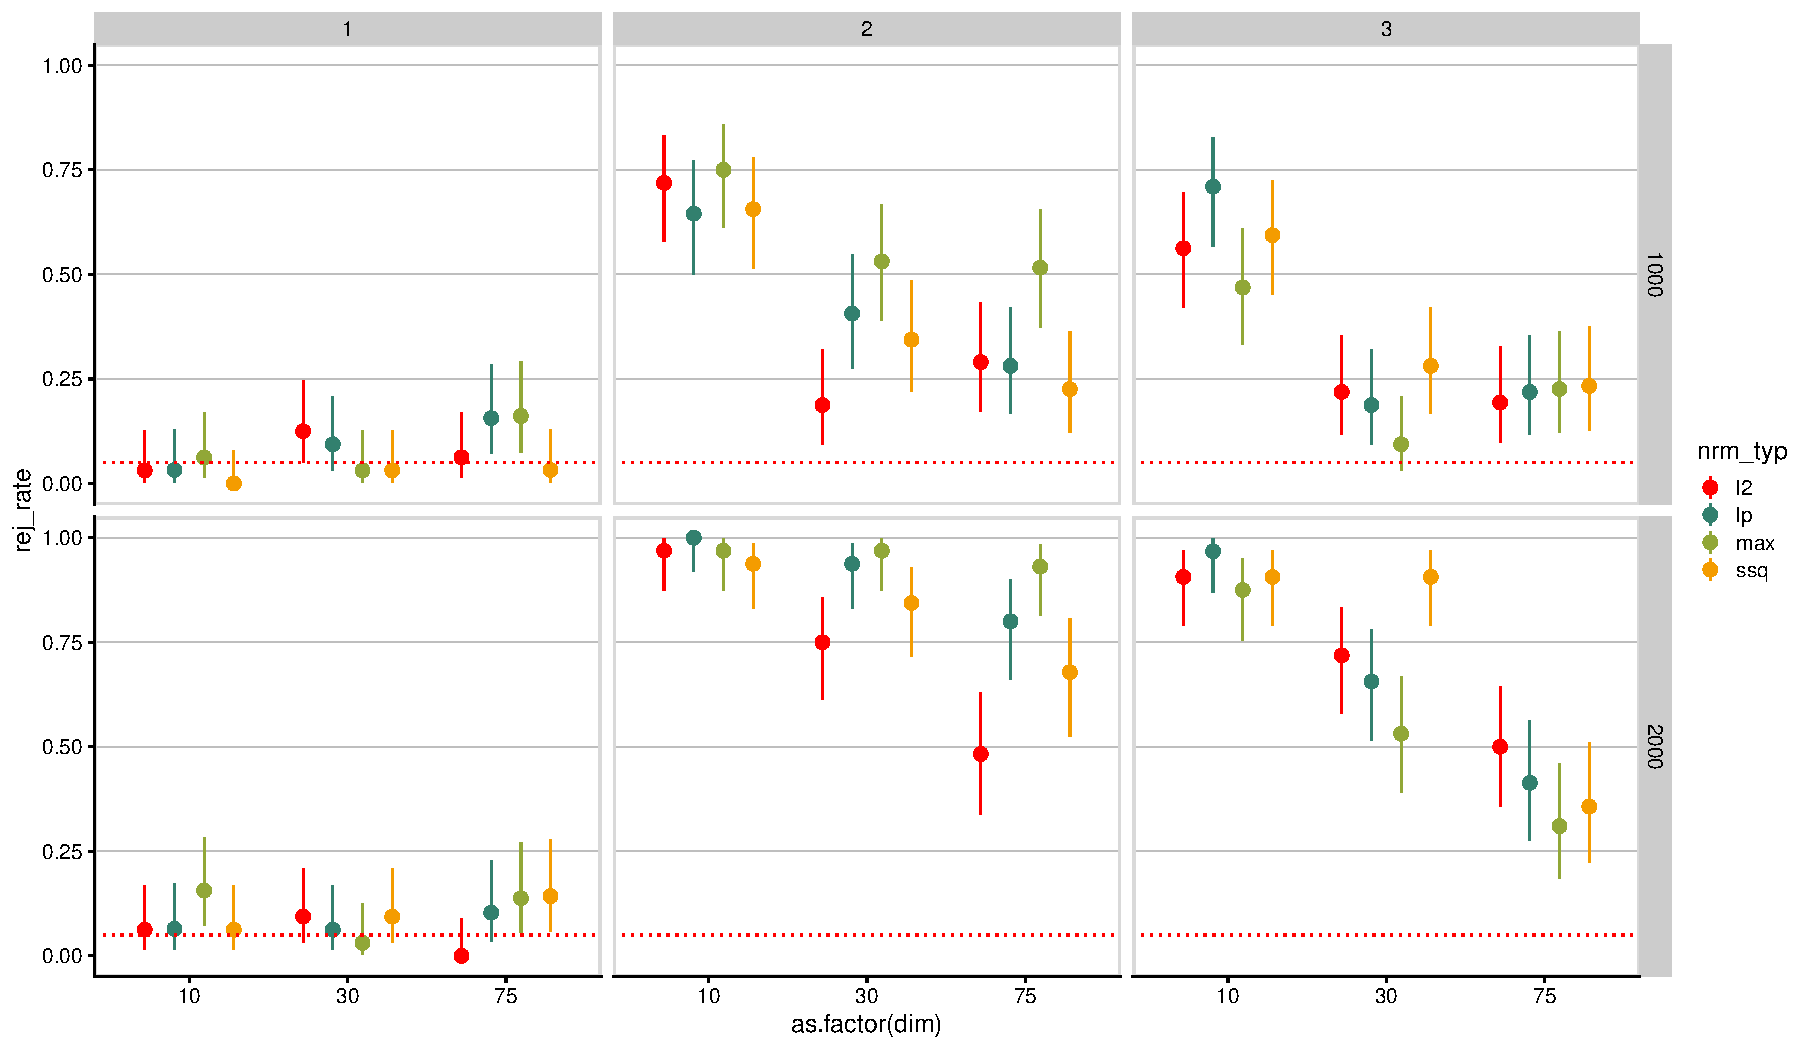
\includegraphics[width = \linewidth]{mag_w_unc_de3.pdf}
	\caption{Rejection rates across a range of settings when a marginal structural model was used to define the parameter of interest.}
	\label{fig:de3}
\end{figure}

Because $H_0$ is true for the first setting, we expect the rejection rates in this setting to be $0.05$.  Figure \ref{fig:de3} show results consistent with this being the case. For the other two settings $H_0$ does not hold so these plots compare the powers between the different testing procedures. While results are not definitive it appears that for the second setting in which a single covariate modifies the treatment effect it appears that the max norm has the best performance followed by the adaptive procedures and then the $\ell_2$ norm. In the third setting in which many covariates are associated with the outcome the adaptive norms appear to once again have middling performance now with the $\ell_2$ norm performing the best and the max norm performing the worst. It was expected that the non-adaptive tests would excel where they did and that the adaptive versions tend to perform well across multiple settings.  It is unclear from these results if, for a given setting, at least one non-adaptive version of the test will outperform the adaptive version of the test.

One setting in which the adaptive test performs poorly is in settings in which a single covariate is correlated with the outcome of interest and no covariates are correlated as seen for model 2 in figure \ref{fig:uncor}. This behavior could be due to the parameter estimates inability to be sparse even in settings when sparsity occurs.  The many small errors in the parameter estimate across many covariates leads to a preference for the $\ell_2$ norm that obtains an overly optimistic estimate of power due to the accumulation of many small effects across all the covariates.


% \section{Data Application}
% \label{sec:data_app}
% \sh{Data from Peter Gilbert}

\section{Discussion}
\label{sec:discuss}
%When developing anything there is frequently a trade off to between generalizability and performance. However the reduction in power of Bonferroni-based methods compared to taylor made procedures is often larger than is needed.  We have developed a generalizable testing procedure that still can outperform Bonferroni based methods.  We have demonstrated this in section \ref{sec:sim_stdy} and shown novel settings in which the method can also be performed.  These settings show that our test can be applied to parameters in non-standard sampling schemes (see section \ref{sec:missing_data}) and complex parameters (see section \ref{sec:msm_data}).  

The general hypothesis testing procedure that we have described relies on asymptotic results to achieve correct type one error rates.  This can cause issues when the number of covariates of interest is larger than the sample size. To address this issue, in certain cases our test can be carried out using permutations of the data to obtain better finite sample properties. 

%\textcolor{blue}{This is done by repeating our estimation procedure many times after randomly permuting the outcome variable.  The method is used in our first data example, and could be used for our third data example. In certain settings with more complicated sampling schemes, the permutation based test is more difficult to implement because many of the outcomes are not even observed.}

% While we have outlined some of the ways in which our method can be used, there are other possible applications and improvements.

While we focused on the studying the limiting distribution of $\sqrt{n}\hat{\psi}$ once can also consider the limiting distribution of $\sqrt{n}\hat{\Sigma}^{-1/2}\hat{\psi}$.  This estimator will always have a multivariate normal limiting distribution with an identity covariance matrix, which simplifies notation by always having a single limiting distribution.  It also simplifies proofs, and potentially could allow for analytical solutions for which norm (or weighted average of norms) would provide the best power.  However, this estimator runs into issues when $p > n$ and $\hat{\Sigma}^{-1/2}$ becomes impossible to estimate because of the rank deficiency of the variance estimator.  While this problem still technically exists when indexing our $\Gamma$s by $\hat{\Sigma}$, using a multiplier bootstrap to take draws from $N(0, \hat{\Sigma})$ avoids the computation issues of having a degenerate estimate of the limiting distributions variance matrix.

\textcolor{blue}{Mention choice of norms and choice of performance metric}

%While changing the test statistic as described above has major hurdles to overcome to be implemented in $p > n$ settings, there are other extensions or generalizations of our procedure that are possible without much change.  While we considered one set of $\Gamma$ functions in this article, any set of reasonable $\Gamma$ functions could be used.  
%These functions could even be picked by machine learning methods used for classification.  The classifier would provide a probability that any observation was generated from the null distribution.  Doing this provides a more rich set of $\Gamma$ over which to select, and has the potential to provide large increases in test performance.  One would expect that a classifier would perform better better when data are generated at an alternative versus at the null.  Thus one could reject when the classification performance is especially large.  

While our procedure currently only selects a single norm to calculate the test statistic, it is possible to also consider an estimator that is a weighted average of the many different norms.  The weights would be estimates of the probability that each norm was optimal. These probabilities could be estimated by taking many draws from a normal with mean $\sqrt{n}\hat{\boldsymbol{\psi}}$ and variance $\hat{\Sigma}$ and finding the optimal norm for each of these draws.  
%This method while being more computationally costly, could potentially be shown theoretically to be optimal in the sense that it would maximize the average power of all tests based on the specified family of norms for each local alternative. 

% While $\ell_p$ norms were used throughout this paper, one issue observed with our test is that it selects the $\ell_2$ norm more frequently than it should, likely because of the many small estimates for parameters that are not associated with the outcome.  One could consider a slightly modified norm that sets to zero all component values of the vector that are less than some value.  This would hopefully solve issues of small values close to zero causing incorrect selection of norms that perform well when there are many small effects.

\textcolor{blue}{add notes about limitation of our method (need to find influence function).  Add notes of computeraization.  Also discuss difficulty with convergence when using the parametric bootstrap.}

% In this article chose tests in which each parameter corresponded to a single covariate, and each covariate only had a single corresponding parameter.  However it would also be possible to have tests where each parameter corresponded to a set of many covariates or each covariate or group of covariates had multiple measures of association.

\section{Conclusion}

\section{Appendix}
This appendix is primarily focused on proving the consistency and local power of our testing procedure.  

For multiple proofs it will be necessary to use the dominated convergence theorem, and find a dominating measure for $\phi(x, \mu, \Sigma)$ and $\phi(x, \mu_n, \Sigma_n)$ where $\phi$ is the pdf for a multivariate normal distribution.


\begin{lemma}
	\label{lemma:dom_measure}
	The function $\phi : \mathbb{R}^d \otimes \mathbb{R}^d \otimes \mathbb{R}^{d \times d} \to \mathbb{R}$ defined by
\begin{align*}
	\phi : (x, \mu, \Sigma) \mapsto \text{det}(\Sigma)^{-1/2}(2\pi)^{-k/2}\text{exp}\left( - \frac{1}{2}(x- \mu)\Sigma^{-1}(x- \mu)\right)
\end{align*}
	is continuous and $\phi_{\Sigma, \mu} : x \mapsto \phi(x, \Sigma, \mu)$ and $\phi_{\mu_n, \Sigma_n} : x \mapsto \phi(x, \Sigma_n, \mu_n)$ are dominated by an integrable function.
\end{lemma}

\begin{proof}
Since matrix inverses, matrix determinants, matrix multiplication, and the exponential function are all continuous, it follows that the multivariate normal distribution is also continuous with respect to $\Sigma, \mu$ and $x$.  Because of this, we also know that for large enough $n$ that 

\begin{align*}
\left|\frac{1}{2}(x_n - \mu_n)\Sigma_n^{-1}(x_n - \mu_n) - \frac{1}{2}(x - \mu)\Sigma^{-1}(x - \mu)\right| < \varepsilon
\end{align*}

for any $\varepsilon$ we choose.  When $\varepsilon = \text{log}(2)$ it is the case that 
% $\max\left(0, 2 \text{log}\left((2 \pi)^{-k} \text{det}(\Sigma)^{1/2}\right)\right)$. 
% We can also bound $\left|\phi(x_n, \mu_n, \Sigma_n) - \phi(x, \mu, \Sigma)\right|$ by 1 for large enough $n$.  For $x, \mu$ such that $\frac{1}{2}(x - \mu)\Sigma^{-1}(x - \mu)/2 < \varepsilon$, we know $\phi(x, \mu, \Sigma) > 1$ therefore. 
% \begin{align*}
% 	\phi(x, \mu_n, \Sigma_n) - \phi(x, \mu, \Sigma) &\leq \left|\phi(x, \mu_n, \Sigma_n) - \phi(x, \mu, \Sigma)\right| \leq 1 \leq \phi(x, \mu, \Sigma)\\
% 	\text{therefore }\phi(x, \mu_n, \Sigma_n) &\leq 2\phi(x, \mu, \Sigma)
% \end{align*}


\begin{align*}
	\frac{\psi(x, \mu_n, \Sigma_n)}{\psi(x, \mu, \Sigma)} &= \frac{\frac{\text{det}(\Sigma_n)^{-1/2}}{(2\pi)^{k/2}}\text{exp}\left( - \frac{1}{2}(x_n - \mu_n)\Sigma_n^{-1}(x_n - \mu_n)\right)}{\frac{\text{det}(\Sigma)^{-1/2}}{(2\pi)^{k/2}}\text{exp}\left( - \frac{1}{2}(x - \mu)\Sigma^{-1}(x - \mu)\right)}\\
	&= \frac{\text{det}(\Sigma_n)^{-1/2}\text{exp}\left(- \frac{1}{2}\left((x_n - \mu_n)\Sigma_n^{-1}(x_n - \mu_n)- (x - \mu)\Sigma^{-1}(x - \mu)\right)\right)}{\text{det}(\Sigma)^{-1/2}} \\
	&\leq \frac{\text{det}(\Sigma_n)^{-1/2}\text{exp}\left( \left| - \frac{1}{2}\left((x_n - \mu_n)\Sigma_n^{-1}(x_n - \mu_n) - (x - \mu)\Sigma^{-1}(x - \mu) \right|\right)\right)}{\text{det}(\Sigma)^{-1/2}} \\
	&\leq \frac{\text{det}(\Sigma_n)^{-1/2}\text{exp}\left(\text{log}(2)\right)}{\text{det}(\Sigma)^{-1/2}} \\
	&\leq \frac{\text{det}(\Sigma_n)^{-1/2} 2 }{\text{det}(\Sigma)^{-1/2}} 
\end{align*}
% For $\frac{1}{2} (x - \mu)\Sigma^{-1}(x - \mu) \geq \varepsilon$ we can do something similar.  First note that for $n$ large enough, 
Next, note that 
\begin{align*}
	\text{det}(\Sigma_n)^{-1/2} - \text{det}(\Sigma)^{-1/2} \leq \left|  \text{det}(\Sigma_n)^{-1/2} - \text{det}(\Sigma)^{-1/2} \right| \leq \text{det}(\Sigma)^{-1/2} \Rightarrow \text{det}(\Sigma_n)^{-1/2} \leq 2\text{det}(\Sigma)^{-1/2}
\end{align*}
Therefore, we find that 
\begin{align*}
	\frac{\text{det}(\Sigma_n)^{-1/2} 2 }{\text{det}(\Sigma)^{-1/2}} &\leq \frac{\left[2\text{det}(\Sigma_n)\right]^{-1/2} 2 }{\text{det}(\Sigma)^{-1/2}} = 2\sqrt{2}
\end{align*}

Thus, for large enough $n$, we can bound $\phi(x, \mu_n, \Sigma_n)$ by $2\sqrt{2} \phi(x, \mu, \Sigma)$ which is integrable.  

% \begin{align*}
% 	\left|\frac{1}{2}(x_n - \mu_n)\Sigma_n^{-1}(x_n - \mu_n) - \frac{1}{2}(x - \mu)\Sigma^{-1}(x - \mu)\right| < \varepsilon &\leq \frac{1}{2}(x - \mu)\Sigma^{-1}(x - \mu) / 2 \\
% 	\frac{1}{2}(x_n - \mu_n)\Sigma_n^{-1}(x_n - \mu_n) & \geq \frac{1}{2}(x - \mu)\Sigma^{-1}(x - \mu)/2\\
% 	\text{exp}\left( - \frac{1}{2}(x_n - \mu_n)\Sigma_n^{-1}(x_n - \mu_n)\right) &\leq \text{exp}\left( - \frac{1}{2}(x - \mu)\Sigma^{-1}/2(x - \mu)\right)\\
% 	\frac{\text{det}(\Sigma_n)^{-1/2}}{(2\pi)^{k/2}}\text{exp}\left( - \frac{1}{2}(x_n - \mu_n)\Sigma_n^{-1}(x_n - \mu_n)\right) &\leq (2\pi)^{-k/2}2\text{det}(\Sigma)^{-1/2}\text{exp}\left( - \frac{1}{2}(x - \mu)\Sigma^{-1}/2(x - \mu)\right)\\
% 	\phi\left(x_n, \mu_n, \Sigma_n\right) &\leq (2\pi)^{-k/2}2\text{det}(\Sigma)^{-1/2}\frac{\text{det}(2\Sigma)^{-1/2}}{\text{det}(2\Sigma)^{-1/2}}\text{exp}\left( - \frac{1}{2}(x - \mu)\Sigma^{-1}/2(x - \mu)\right)\\
% 	&=\frac{\text{det}(2\Sigma)^{-1/2}}{(2\pi)^{k/2}}\frac{2\text{det}(\Sigma)^{-1/2}}{2^{-k/2}\text{det}(\Sigma)^{-1/2}}\text{exp}\left( - \frac{1}{2}(x - \mu)\Sigma^{-1}/2(x - \mu)\right)\\
% 	&=\frac{\text{det}(2\Sigma)^{-1/2}}{(2\pi)^{k/2}}2^{1 + k/2}\text{exp}\left( - \frac{1}{2}(x - \mu)\Sigma^{-1}/2(x - \mu)\right)\\
% 	&=2^{k/2 + 1}\phi(x, \mu, 2\Sigma)\\
% e\end{align*}

% Thus, we know that we can bound both $\phi(x, \mu, \Sigma)$ and $\phi(x_n, \mu_n, \Sigma_n)$ by the function: 

% \begin{align*}
% 	\zeta(x, \mu, \Sigma) = 2\phi(x, \mu, \Sigma) + 2^{k/2 + 1} \phi(x, \mu, 2\Sigma)
% \end{align*}

% Which we know is integrable with respect to $x \in \mathbb{R}^d$ because it is a linear combination of two integrable functions.
\end{proof}

\begin{lemma}
	\label{lemma:gamma_conv}
	Let $\hat{Z} \sim N(0, \hat{\Sigma})$ and $Z \sim N(0, \Sigma)$. If $\hat{\Sigma}$ is a consistent estimator of $\Sigma$, $\Gamma : \mathbb{R}^{d} \otimes \mathbb{R}^{d^2}$ is continuous, and $Pr(\Gamma(Z, \Sigma) = t) = 0$ for each $t$.  It follows that the distribution function of $\Gamma(\hat{Z}, \hat{\Sigma})$ denoted by $F_{\Gamma(\hat{Z}, \hat{\Sigma})}$ converges pointwise to the distribution function of $\Gamma(Z, \Sigma)$ denoted by $F_{\gamz}$ and the quantile function of $\gamestz$ denoted by $F^{-1}_{\gamestz}$ converges pointwise to the quantile function of $\gamz$ denoted $F^{-1}_{\gamz}$ where $F^{-1} : [0, 1] \to \mathbb{R}$ is defined By $F^{-1}(p) = \inf\{x : F(x) \geq p\}$
\end{lemma}

\begin{proof}
	From Lemma \ref{lemma:dom_measure} we know that we there exists a dominating function for the probability density functions of $\hat{Z}$ and $Z$. Applying dominated convergence theorem shows that 
	\begin{align*}
		\text{Pr}\left(\Gamma(\hat{Z}, \hat{\Sigma}) \leq t \right) = \int I\{\Gamma(x, \hat{\Sigma}) \leq t\} \phi(x, \hat{\mu}, \hat{\Sigma}) dx \rightarrow \int I\{\Gamma(x, \Sigma) \leq t\} \phi(x, \mu, \Sigma) dx = \text{Pr}\left(\Gamma(Z, \Sigma)) \leq t \right).
	\end{align*}
The convergence of the distribution functions shown above and lemma 21.1 of \citep{van_der_vaart_asymptotic_2000} imply the pointwise convergence of the corresponding quantile functions.
\end{proof}

\subsection{Proof of Theorem \ref{thm:cnst} (Test Consistency)}
\begin{proof}
Let $Z \sim N\left(\boldsymbol{0}, \Sigma\right)$ and  $\hat{Z} \sim N\left(\boldsymbol{0}, \hat{\Sigma}\right)$.
Lemma \ref{lemma:gamma_conv} and the assumptions of the theorem imply the pointwise convergence of the distribution function of $\gamestz$ denoted by $F_{\gamestz}$ to the distribution function of $\gamz$ denoted by $F_{\gamz}$ and the pointwise convergence of the quantile function of $F_{\gamestz}$ to the quantile function of $F_{\gamz}$. By the assumption of the theorem $F^{-1}_{\gamz}(\alpha) > 0$, so

\begin{align*}
	\text{Pr}_{P}\left(\gamestp \leq F^{-1}_{\gamestz}(\alpha)\right) &= 1 - \text{Pr}_{P}\left(\gamestp \geq F^{-1}_{\gamestz}(\alpha)\right)\\
	& \geq 1 - \frac{E\left[|\gamestp|\right]}{F^{-1}_{\gamestz}(\alpha)} \xrightarrow{p} 1.
\end{align*}
\end{proof}

While $\Gamma(x, \Sigma)$ may not grow close to zero as $x$ becomes large, one can use transformations of the original $\Gamma$ to achieve this property.  
% Note that this property is implicitly dependent on choice of norms.
We show that the performance metrics used in this paper satisfy the satisfy conditions 1-3 in lemmas \ref{lemma:est_accept} and \ref{lemma:mult_dist_gam}. 

\subsection{Unbiasedness at local alternatives}
To prove non-trivial local unbiasedness, we rely heavily on a result of \citep{eaton_multivariate_1991}. It states that for two centrally symmetric, unimodal functions, $f_1$ and $f_2$, the function $g : \mathbb{R}^d \mapsto \mathbb{R}$ defined by the convolution:  
	\begin{align*}
		g(\underline{h}) = \int f_1(x) f_2(x - \underline{h})
	\end{align*}
	is centrally symmetric and ray decreasing.  A function $f :\mathbb{R}^p\rightarrow\mathbb{R}$ is centrally symmetric if $f(-x) = f(x)$ for every $x$.  A function is unimodal if for every $k$, the set $\{x : f(x) \geq k\}$ is convex. A function $f$ on $\mathbb{R}^p$ is ray decreasing if for every $x$ in $\mathbb{R}^p$, the function $g(\beta) = f(\beta x), \beta \in \mathbb{R}^+$ is a non-increasing function of $\beta$.  Additional conditions are required to hold for $g(\beta)$ to be a strictly decreasing function of $\beta$.  These conditions are shown to hold in lemma \ref{lemma:aditional_anderson_cond} for $\Gamma$ that satisfy conditions 1, 2, 4, and 5.  

Our testing procedure can be rewritten in using the above form, where $f_1(x)$ is $I\{\Gamma^*_{\vmat}(x) > F^{-1}_{\Gamma^*_{\vmat}(\rvv)}(\alpha)\}$, and $f_2$ is a multivariate pdf with mean $0$.  The ray decreasing quality of $g$ can then be used to show that 

\begin{align*}
	Pr_{\disto}\left(\Gamma(Z + \underline{h}, \Sigma) \leq F^{-1}_{\Gamma(\rvv, \Sigma)}(\alpha)\right) > Pr_{\disto}\left(\gamz \leq F^{-1}_{\gamz}(\alpha)\right) = \alpha
\end{align*}

Because the multivariate normal pdf is centrally symmetric and unimodal (see lemma \ref{lemma:mvtnorm_unimodality}), all that remains to be shown is that the function $(x, \Sigma) \mapsto I\{\Gamma(x, \Sigma) > F^{-1}_{\gamz}(\alpha)\}$ is unimodal and centrally symmetric.  Lemma \ref{lemma:indct_cent_sym_unm} tells us that this indicator function is unimodal if $\Gamma$ is unimodal and centrally symmetric.  

In lemmas \ref{lemma:est_accept} and \ref{lemma:mult_dist_gam}, we show that the $\Gamma$ used in this article are unimodal and centrally symmetric.

\subsection{Proof of Theorem \ref{thm:unbiased_locl_alt} (Non-Trivial Local Unbiasedness)}

\begin{proof}
Lemma \ref{lemma:gamma_conv} and the assumptions of the theorem imply the pointwise convergence of the distribution function of $\gamestz$ denoted by $F_{\gamestz}$ to the distribution function of $\gamz$ denoted by $F_{\gamz}$ and the pointwise convergence of the quantile function of $F_{\gamestz}$ to the quantile function of $F_{\gamz}$.  Thus
% Thus, letting $c_\alpha = F^{-1}_{\Gamma^*_{\vmat}(\rvv)}(\alpha)$ we find

\begin{align*}
	Pr_{\disto}\left(\gamestp \leq F^{-1}_{\gamestz}(\alpha)\right) \xrightarrow{p} Pr_{\disto}\left(\Gamma(Z + \underline{h}, \vmat) \leq F^{-1}_{\gamz}(\alpha)\right).
\end{align*}

Breaking down the quantity on the right, the only random part inside of the probability statement is $Z$.  Define the function $g^* : \mathbb{R}^d \to \mathbb{R}$ by the quantity inside the probability statement on the right hand side of the the above display:

\begin{align}
	g(\underline{h}) = Pr_{\disto}\left(\Gamma(Z + \underline{h}, \Sigma) \leq F^{-1}_{\gamz}(\alpha)\right)  &= \int I\left\{\Gamma(x, \Sigma) \leq c_\alpha\right\} \phi(x - \underline{h}) dx \nonumber \\
	&=  \int \left(1 - I\left\{\Gamma(x, \Sigma) \geq c_\alpha \right\}\right)\phi(x - \underline{h}) dx \nonumber\\
	&= 1 - \int I\left\{\Gamma(x, \Sigma) \geq c_{\alpha}\right\} \phi(x - \underline{h}) dx. \label{eqn:decreasing_part}
\end{align}
Because $\Gamma$ is unimodal and centrally symmetric it follows from Lemma \ref{lemma:indct_cent_sym_unm} that $I\left\{\Gamma(x, \Sigma) \geq c_{\alpha}\right\}$ is also centrally symmetric and unimodal. Thus, the subtracted quantity in \eqref{eqn:decreasing_part} is ray decreasing with respect to $\underline{h}$ by \citep{anderson_integral_1955} and attains it maximum at $\underline{h} = 0$.  To show that $g(\underline{h}a)$ is increasing for $a \in [0, 1]$ and $g(\underline{h}) > g(0)$ where \begin{align*}
	g(0) = Pr_{\disto}\left(\gamz \leq F^{-1}_{\gamz}(\alpha)\right),
\end{align*}
The asymptotic probability of rejecting $H_0$ when $H_0$ holds.
\end{proof}

\subsection{Extension of results from $\Gamma$ to $\Gamma^*$}

While theorems \ref{thm:cnst} and \ref{thm:unbiased_locl_alt} place conditions on our adaptive estimator $\Gamma^*$, it may be difficult to directly prove conditions 2-6 hold for $\Gamma^*$.  Here we show that if conditions 2-6 hold for each $\Gamma_1, \dots, \Gamma_k$ and $\Gamma^*(x) = \max\{\Gamma_{1}(x), \dots, \Gamma_{k}(x)\}$, then conditions 2-6 also hold for $\Gamma^*$.

\begin{lemma}
	Let $\Gamma_{1}, \dots, \Gamma_{Sigma, k}$ be such that each $\Gamma_{i}$ is continuous with respect to $x$ and $\Sigma$ is non-negative, and  at least one $\Gamma_{j}$ has the property that $E\left[\Gamma_{j}(\sqrt{n}\hat{\boldsymbol{\psi}}, \hat{\Sigma})\right] \rightarrow 0$ for all fixed $P \not \in \mathcal{M}_0$.  Then if $\Gamma(x) = \max\{\Gamma_{1}(x), \dots, \Gamma_{k}(x)\}$ satisfies conditions 2-4.
\end{lemma}

\begin{proof}
	Because the max function is continuous and the composition of continuous functions is also continuous it follows that $\Gamma^*(x) = \max\{\Gamma_{1}(x), \dots, \Gamma_{k}(x)\}$ is also continuous.  
	Because $\Gamma_{i}(Z) = 0$ for every $i \in \{1, \dots, k\}$, it follows that 
	\begin{align*}
		\text{Pr}(\Gamma^*(Z, \Sigma) = 0) = \text{Pr}\left(Z \in \bigcup_{i = 1}^k \left\{ \omega : \Gamma_{i}(\omega, \Sigma) = 0 \right\} \right) \leq \sum_{i = 1}^k \text{Pr}(\Gamma_{\Sigma, 1}(Z) = 0) = 0 
	\end{align*}
\end{proof}

\begin{lemma}
	\label{lemma:min_cent_sym_unm}
	Let $\Gamma_{1}, \dots, \Gamma_{k}$ all be centrally symmetric, unimodal functions.  Then $\Gamma^* = \min\left\{\Gamma_{1}, \dots, \Gamma_{k}\right\}$ is also centrally symmetric and unimodal.
\end{lemma}
\begin{proof}
Because each $\gi_i$ is a centrally symmetric and $\gi^*$ is a function of $x$ only through $\gi_i$ it follows that $\gi^*$ is also centrally symmetric:
	\begin{align*}
	\gi^*(x) = \min\left\{\gi_1(x), \dots, \gi_k(x)\right\} = \min\left\{\gi_1(-x), \dots, \gi_k(-x)\right\} = \gi^*(-x)
	\end{align*}
The set $M^* \equiv \{x : \Gamma^*(x) \geq k\}$ contains all of the $x$ for which $\Gamma \geq k$ for all $i \in \{1, \dots, d\}$.  Thus $M^*$ is the intersection of all sets $M_i \equiv \{x : \Gamma_{i}(x) \geq k\}$.  Each $M_i$ is convex because each $\Gamma_{i}$ is unimodal, and the intersection of a countable number of convex sets is convex.  Thus $M^*$ is convex and $\Gamma_{\Sigma}^*$ is unimodal.
	% \begin{align*}
	% 	\left\{x : \gi^*(x) \geq k\right\} = \left\{x : \gi_1(x) \geq k, \dots, \gi_d(x) \geq k\right\} = \bigcap_{i = 1}^d \left\{x : \gi_i(x) \geq k \right\}
	% \end{align*}
\end{proof}


\subsection*{Performance Metric Specific proofs}
In this section, we show that both performance metrics we consider satisfy conditions 2-6. This requires setting conditions on the norms that index the performance metrics. The requirements we place on the norms are that
\begin{itemize}
	\item each norm obeys the triangle inequality: $\|x\|_p + \|y\|_p \geq \|x + y\|_p$ for every $x$ and $y$ in $\mathbb{R}^d$
	\item For each $\omega \in \mathbb{R}$, the set $\left\{x : \|x\| < \omega\right\}$ is convex.
	\item each norm has a gradient which is finite at $\psi$ for all possible values of $\psi$.
\end{itemize}

The second requirement mentioned above will allow us to bound the variance of the normed vector of parameter estimators as described in the following lemma.  This fact will be used to prove both condition 4 ($E\left[\gamestp \right] \rightarrow 0$ for all fixed $P \not \in \mathcal{M}_0$.) for both performance metrics.  

\begin{lemma}
	Let $\hat{Z} \sim N(0, \hat{\Sigma})$ with $\hat{\Sigma} \xrightarrow{p} \Sigma$ be independent of $\hat{\boldsymbol{\psi}}$ for every $n$, and $\tst \xrightarrow{p} N(0, \Sigma)$.  If $||\cdot||_p$ has a finite derivative at $\boldsymbol{\psi}$ then 

	\begin{align*}
		\text{var}\left(\left\|\hat{Z} + \sqrt{n}\left(\hat{\boldsymbol{\psi}} - \boldsymbol{\psi}\right) \right\|_p\right) \leq M
	\end{align*}
	for some $M$.
\end{lemma}

\begin{proof}
	Because of the independence of the two random variables, and the convergence in distribution of $\sqrt{n}\left(\hat{\boldsymbol{\psi}} - \boldsymbol{\psi}\right)$, we know that
	\begin{align*}
		\hat{Z} + \sqrt{n}\left(\hat{\boldsymbol{\psi}} - \boldsymbol{\psi}\right) =  \sqrt{n}\left(\hat{\boldsymbol{\psi}} + \frac{\hat{Z}}{\sqrt{n}} - \boldsymbol{\psi}\right) \xrightarrow{d} Z^* \sim N(0, \sqrt{2} \Sigma)
	\end{align*}
	Thus, the delta method tells us that
	\begin{align*}
		\|\hat{Z} + \sqrt{n}\left(\hat{\boldsymbol{\psi}} - \boldsymbol{\psi}\right)\|_p \xrightarrow{d} \|Z^*\|_p \sim N\left(0, \nabla\|\boldsymbol{\psi}\|_p^\top \sqrt{2}\Sigma \nabla\|\boldsymbol{\psi}\|_p \right)
	\end{align*}
	Because the gradient of $\|\cdot\|_p$ is bounded at $ \boldsymbol{\psi}$, the variance of $\|Z^*\|_p$ will be bounded as well.
\end{proof}

\subsubsection{Estimated Acceptance Rate}

\begin{lemma}
	\label{lemma:est_accept}
	The function $\Gamma : \mathbb{R}^d \otimes \mathbb{R}^{d \times d} \to \mathbb{R}$ defined by 
	\begin{align*}
		\Gamma(t, \Sigma) = Pr_\distv(\|\tilde\rvv + t\| < c_{0.8})  \text{ where }  c_{\vmat, 0.8} \equiv \min_{c}\{c : Pr_\distv(\|\tilde\rvv\| < c) \geq 0.8 \} \text{ and } \tilde\rvv \sim N(0, \Sigma)
	\end{align*}
	satisfies conditions 1 - 5.
\end{lemma}

\begin{proof}

\textbf{Continuity:}
Because $\Gamma$ is the integral of a function (namely the multivariate normal probability density function) that is continuous with respect to both $\Sigma$ and $x$ (see Lemma \ref{lemma:dom_measure}), it follows that $\Gamma$ is also continuous. 

\textbf{$\pr\left(\gamz = t\right) = 0$ for each $t$:}
Because $Z$ and $\tilde{Z}$ are both normally distributed the probability mass functions of both random variables are positive over the entirety of $\mathbb{R}^d$.  Considering the set of values $\left\{\omega : \|\omega\| = t\right\}$, the probability any normal random variable falls within this region is some positive value no matter what the mean of the random variable is.  Therefore, $\pr\left(\gamz = 0\right) = 0$. 

\textbf{Convergence of $\Gamma_{\hat{\Sigma}}(\sqrt{n}\hat{\boldsymbol{\psi}})$ to zero under fixed alternatives:}
\begin{align*}
	E[|\gamestp|] &= E\left[ |\text{Pr}(\|\hat{Z} + \tst \|\leq c_\alpha) |\right]\\
	&= E\left[E\left(I\left\{\|\hat{Z} + \tst\|_p \leq c_\alpha\right\} \right)\right]\\
	&= E\left[I\left\{\|\hat{Z} + \sqrt{n}\hat{\boldsymbol{\psi}} \|_p \leq c_\alpha\right\} \right]  = \text{Pr}_{P}\left(\|\hat{Z} + \tst\|_p \leq c_\alpha\right) \\
	& = \text{Pr}_{P}\left(\|\hat{Z} + \sqrt{n}\left(\hat{\boldsymbol{\psi}} - \boldsymbol{\psi}\right) + \sqrt{n} \boldsymbol{\psi}\|_p \leq c_\alpha\right) \\
	& \leq \text{Pr}_{P}\left(\|\sqrt{n} \boldsymbol{\psi}\|_p - \|\hat{Z} + \sqrt{n}\left(\hat{\boldsymbol{\psi}} - \boldsymbol{\psi}\right)\|_p  \leq c_\alpha\right) \\
	& = \text{Pr}_{P}\left(\|\sqrt{n} \boldsymbol{\psi}\|_p -  c_\alpha \leq \|\hat{Z} + \sqrt{n}\left(\hat{\boldsymbol{\psi}} - \boldsymbol{\psi}\right)\|_p\right) \\
	& \leq \frac{\text{var}\left(\|\hat{Z} + \sqrt{n}\left(\hat{\boldsymbol{\psi}} - \boldsymbol{\psi}\right)\|_p \right)}{\|\sqrt{n} \boldsymbol{\psi}\|_p -  c_\alpha}\\
\end{align*}
Since the numerator converges to a finite value, and the denominator grows without bound, we know the fraction as a whole will converge to zero.

\textbf{Central Symmetry:}
Because the multivariate normal distribution is centrally symmetric, so is $\Gamma(t, \Sigma)$:

\begin{align*}
	\Gamma(\mu, \Sigma) = \int I\left\{\|x\|_p < c\right\} \phi_{\Sigma}(x - \mu)dx &= \int I\left\{\|x + \mu\|_p < c\right\} \phi_{\Sigma}(x))dx \\
	&= \int I\left\{\|x + \mu\|_p < c\right\} \phi_{\Sigma}(-x))dx\\
	&= \int I\left\{\|x\|_p < c\right\} \phi_{\Sigma}(-x - \mu))dx\\
	&= \int I\left\{\|x\|_p < c\right\} \phi_{\Sigma}(x + \mu))dx\\
	&= \Gamma(-\mu, \Sigma)
\end{align*}

\textbf{Unimodality: }
First note that

\begin{align*}
	\Gamma(\mu, \Sigma) & = \int I\left\{\|x\|_p < c\right\} \phi_{\Sigma}(x - \mu)dx = \int I\left\{\|x + \mu\|_p < c\right\} \phi_{\Sigma}(x)dx = P(Z \in A_\mu) \equiv P_Z(A_\mu)
\end{align*}

Where $Z \sim N(0, \Sigma)$ and $A_\mu = \{t : \|t + \mu\| < c\}$

Next consider $\mu_1, \mu_2$ such that $\Gamma(\mu_1, \Sigma) \geq k$, and $\Gamma(\mu_2, \Sigma) \geq k$. Because the multivariate normal pdf is log concave (Theorem 4.2.1 of \citep{tong_multivariate_2012}), we can apply theorem 1 of \citep{rinott_convexity_1976} to obtain the result that:
\begin{align*}
	k = k^{t}k^{1 - t} \leq \Gamma(\mu_1, \Sigma)^t \Gamma(\mu_2, \Sigma)^{1 - t} =  P_Z(A_{\mu_1})^tP_Z(A_{\mu_2})^{1 - t} \leq P_Z(tA_{\mu_1} + (1 - t) A_{\mu_2}).
\end{align*}
Lemma \ref{lemma:set_convexity} shows that $tA_{\mu_1} + (1 - t) A_{\mu_2} = A_{t\mu_1 + (1 - t) \mu_2}$ so it follows that
\begin{align*}
	P_Z(tA_{\mu_1} + (1 - t) A_{\mu_2}) = P_Z(A_{t\mu_1 + (1 - t) \mu_2}) = \Gamma_{\Sigma}(t\mu_1 + (1 - t) \mu_2)
\end{align*}

\end{proof}

\textbf{Multiplicative distance performance metric}
\textcolor{red}{Still need to show continuity and condition 3 hold for this performance metric}

Consider the other measure of performance we have used: 

\begin{lemma}
	\label{lemma:mult_dist_gam}
	The function $\Gamma : \mathbb{R}^d \otimes \mathbb{R}^{d^2} \mapsto (0, \infty)$ defined by
	\begin{align*}
		\Gamma(t, \Sigma) = \text{min}\left\{s : \text{Pr}(\|Z + st\|_p \geq c_\alpha) \geq 0.8 \right\}
	\end{align*}
	satisfies conditions 1-5.
\end{lemma}

\begin{proof}
\textbf{Continuity}

\textbf{$\gamz$ has measure zero at zero.}
	Because $c_{\alpha}$ is defined in such a way that $\text{Pr}(\|Z\|_p \geq c_\alpha) \leq 0.2 < 0.8$, and because $0 \times t = 0$ for any real-valued $t$, the probability that $\Gamma^*(Z, \Sigma) = 0$ is 0.

\textbf{$E\left[|\gamestp|\right]$ converges to zero for fixed alternatives:}

Consider the sequence of $s_n^* = n^{- 1/4}$

\begin{align*}
 \text{Pr}(\|\hat{Z} + s_n^{*}\tst\|_p \geq c_\alpha) &= \text{Pr}\left(\left\|\hat{Z} + n^{-1/4}\left[\sqrt{n}\left(\hat{\boldsymbol{\psi}} - \boldsymbol{\psi} + \boldsymbol{\psi}\right)\right]\right\|_p \geq c_\alpha\right)\\
 &= \text{Pr}\left(\left\|\hat{Z} + n^{-1/4}\left(\hat{\boldsymbol{\psi}} - \boldsymbol{\psi}\right) + n^{1/4}\boldsymbol{\psi}\right\|_p \geq c_\alpha\right)\\
 &\geq \text{Pr}\left( \|n^{1/4}\boldsymbol{\psi}\|_p - \left\|\hat{Z} + n^{1/4}\left(\hat{\boldsymbol{\psi}} - \boldsymbol{\psi}\right) \right\|_p \geq c_\alpha\right)\\
 & = 1 - \text{Pr}\left( \|n^{1/4}\boldsymbol{\psi}\|_p - c_\alpha \leq \left\|\hat{Z} + n^{1/4}\left(\hat{\boldsymbol{\psi}} - \boldsymbol{\psi}\right) \right\|_p \right)\\
 & \geq 1 - \frac{\text{var}\left(\left\|\hat{Z} + n^{1/4}\left(\hat{\boldsymbol{\psi}} - \boldsymbol{\psi}\right) \right\|_p\right)}{\|n^{1/4}\boldsymbol{\psi}\|_p - c_\alpha} 
\end{align*}
Since the denominator of the second term grows without bound, we know the above quantity will tend to 1. Because  $\gamestp$ takes the smallest $s$ such that $\text{Pr}(\|\hat{Z} + s\tst\|_p \geq c_\alpha) \geq 0.8$, and the chosen sequence satisfies $\text{Pr}(\|\hat{Z} + s_n^*\tst\|_p \geq c_\alpha) \rightarrow 1$ it follows that $\gamestp$ must be least as small as $s_n^*$ for large $n$.   Thus for large $n$ it follows that $E\left[|\Gamma(\tst, \Sigma) | \right] \leq E\left[s_n^*\right]\rightarrow 0$

\textbf{Central Symmetry}
	Lemma \ref{lemma:est_accept} showed that the function $f(y) =  \text{Pr}(\|Z + y\|_p \geq c)$ is centrally symmetric and unimodal for any $c$.  

	Therefore, $\Gamma$ is also centrally symmetric:
	\begin{align*}
		\Gamma(-x, \Sigma) = \text{min}\left\{s : \text{Pr}(\|Z + -sx\|_p \geq c_\alpha) \geq 0.8 \right\} = \text{min}\left\{s : \text{Pr}(\|Z + sx\|_p \geq c_\alpha) \geq 0.8 \right\} = \Gamma(x, \Sigma)
	\end{align*}

	\textbf{Unimodality: }
	To show unimodality, consider $\mu_1$ and $\mu_2$ such that $\Gamma(\mu_1, \Sigma)$ and $\Gamma(\mu_2, \Sigma) \geq k$.  Let $s = \text{max}(s_1, s_2)$.  Theorem \ref{thm:unbiased_locl_alt} and lemma \ref{lemma:est_accept} tell us that $\text{Pr}(\|Z + sx\|_p \geq c_\alpha)$ is increasing in $s$, so if $\Gamma(\mu, \Sigma) \geq k$ then $\text{Pr}(\|Z + k\mu\|_p \geq c_\alpha) \geq 0.8$.  This means 
	\begin{align*}
		&\text{Pr}(\|Z + k\mu_1\|_p \geq c_\alpha) \leq 0.8 \text{ and } \text{Pr}(\|Z + k\mu_2\|_p \geq c_\alpha) \leq 0.8\\
		\text{ or equivalently }& \text{Pr}(\|Z + k\mu_1\|_p < c_\alpha) > 0.2 \text{ and } \text{Pr}(\|Z + k\mu_2\|_p < c_\alpha) > 0.2
	\end{align*}
	it follows from lemma \ref{lemma:est_accept} that 
	\begin{align*}
		&\text{Pr}(\|Z + k (t\mu_1 + (1 - t)\mu_2)\|_p < c_\alpha) > 0.2\\
	\text{ or quivalently }	&\text{Pr}(\|Z + k (t\mu_1 + (1 - t)\mu_2)\|_p \geq c_\alpha) \leq 0.8
	\end{align*}
	Thus $\Gamma(t\mu_1 + (1 - t)\mu_2, \Sigma) \geq k$ as well.
\end{proof}

\subsection{Short, but important lemmas}

\begin{lemma}
	\label{lemma:mvtnorm_unimodality}
	The multivariate normal probability density function is unimodal for all $\Sigma$.  
\end{lemma}

\begin{proof}
	Suppose that both $\phi(\mu_1)$ and $\phi(\mu_2) \geq k$.  Because the multivariate normal probability density function is log concave \citep{tong_multivariate_2012}, it follows that 
\begin{align*}
	\log\left(\phi(t \mu_1 + (1 - t) \mu_2)\right) & \geq t\log\left(\phi(\mu_1)\right) + (1 - t) \log\left((\phi(\mu_2)\right)
\end{align*}
Also, since $e^x$ is a strictly increasing function, this would imply:
\begin{align*}
	\exp\left(\log\left(\phi(t \mu_1 + (1 - t) \mu_2)\right)\right) & \geq \exp \left(t\log\left(\phi(\mu_1)\right) + (1 - t) \log\left(\phi(\mu_2)\right) \right)\\
	\phi(t \mu_1 + (1 - t) \mu_2) &\geq \phi(\mu_1)^{t} \phi(\mu_2)^{1-t}\geq k^{t}k^{1 - t} = k
\end{align*}
\end{proof}


\begin{lemma}
	\label{lemma:indct_cent_sym_unm}
	Let $f(x)$ be a centrally symmetric, unimodal function.  Then $g(x) = I\left\{f(x) \geq c\right\}$ where $c \in \mathbb{R}$ is also centrally symmetric and unimodal. 
\end{lemma}
\begin{proof}
Because $f$ is centrally symmetric and $g$ is a function of $x$ only through $g$, $g$ is also centrally symmetric:
	\begin{align*}
	g(x) = I\left\{f(x) \geq c\right\} = I\left\{f(-x) \geq c\right\} = g(-x)
	\end{align*}

	If $k < 0$ or $k > 1$, then $\left\{x : g(x) \geq k\right\}$ will be the empty set or all of $\mathbb{R}^d$ respectively, and both sets are convex.  
	
	Otherwise, the set $\left\{x : g(x) \geq k\right\} = \left\{x : I\left\{f(x) \geq c\right\} \geq k\right\}$. The indicator function will be greater than or equal to $k$ whenever $f(x) \geq c$, so $\left\{x : g(x) \geq k\right\} =\left\{x : f(x) \geq c\right\}$
	which is convex because $f$ is unimodal.

	Thus $g$ is unimodal.
\end{proof}

\begin{lemma}
	\label{lemma:set_convexity}
	If the set $A$ is convex, and if $A_\mu = \{a + \mu : a \in A\}$, then the set $t A_{\mu_1} + (1 - t) A_{\mu_2} = \{b : b = ta_{\mu_1} + (1 - t)a_{\mu_2}, a_{\mu_1} \in A_{\mu_1}, a_{\mu_2} \in A_{\mu_2}\}$ is equivalent to $A_{t\mu_1 + (1 - t) \mu_2}$
\end{lemma}
\begin{proof}
	Let $x \in t A_{\mu_1} + (1 - t) A_{\mu_2}$.  Therefore
	\begin{align*}
		x &= a_{\mu_1}t + a_{\mu_2}(1 - t) \text{ where } a_{\mu_1} \in A_{\mu_1}, a_{\mu_2} \in A_{\mu_2}\\
		 &= (a_1 + \mu_1) t + (a_2 + \mu_2)(1 - t) \text{ where } a_1, a_2 \in A\\
		 &= a_1 t + a_2 (1 - t) + \mu_1 t + \mu_2 (1 - t) \text{ where } a_1, a_2 \in A\\
	\end{align*}
	Because of the convexity of $A$ it follows that $a_1 t + a_2 (1 - t)$ and $x \in A_{\mu_1 t + \mu_2 (1 - t)}$.  To show inclusion in the reverse direction, let $y \in A_{\mu_1 t + \mu_2 (1 - t)}$.  Then:
	\begin{align*}
		y &= a + \mu_1 t + \mu_2 (1 - t) \text{ where } a \in A\\
		 &= (a + \mu_1) t + (a + \mu_2) (1 - t) \text{ where } a \in A
	\end{align*}
	so $y \in t A_{\mu_1} + (1 - t) A_{\mu_2}$.
\end{proof}

\subsection*{Additional conditions for Anderson Theorem}
In order to show a strict inequality 

\begin{align*}
\int I\left\{\Gamma(x, \Sigma) \geq c_{\alpha}\right\} \phi(x - \underline{h}) dx = \int I\left\{\Gamma(x + \underline{h}, \Sigma) \geq c_{\alpha}\right\} \phi(x ) dx  < \int I\left\{\Gamma(x, \Sigma) \geq c_{\alpha}\right\} \phi(x) dx \label{eqn:decreasing_part} 
\end{align*}


it must be shown that for at least one $u$, $K_u = \left\{ x : \phi(x) \geq u\right\}$ and $H_h = \left\{x : \Gamma(x + \underline{h}, \Sigma) \geq c_\alpha\right\}$ that the volume of $\left\{K_u \cap H_h \right\}$ is less than $\left\{K_u \cap H_0 \right\}$. 

\begin{lemma}
	The above condition holds for all $\Gamma$ satisfying conditions 1 - 5. \label{lemma:aditional_anderson_cond}
\end{lemma}

\begin{proof}
	Because the set $H_0$ is closed and bounded, let $x_0 \in \text{argmin}\left\{\phi(x) : x \in H_0\right\}$. 
	Now, consider the equivalent point inside of $H_h$ which is the point $x_0 + \underline{h}$.  Comparing these two values, compare:
	\begin{align*}
		x_0^{\top}\Sigma^{-1}x_0 \text{ v.s. } (x_0 + \underline{h})^{\top}\Sigma^{-1}(x_0 + \underline{h}) = x_0^\top\Sigma^{-1}x_0 + 2 \underline{h}^{\top}\Sigma^{-1}x_0 + \underline{h}^{\top}\Sigma\underline{h}
	\end{align*}
	If the value of $2 \underline{h}^{\top}\Sigma^{-1}x_0$ is negative, instead consider $-x_0$.  Because $\phi$ is centrally symmetric we now that $-x_0 \in \text{argmin}\left\{\phi(x) : x \in H_0\right\}$ as well. 
	Thus it is the case that $\phi(x_0) > \phi(x_0 + \underline{h}_0)$.  Also, because $\phi$ is continuous, it is also true that for some $\delta$ all $x \in B(x_0 + \underline{h}, \delta) = \left\{y : |y - x_0 + \underline{h}| < \delta \right\}$ that $\phi(x) < \phi(x_0)$.  

	Because $H_0$ has a positive volume, we know that there exists a set of points $\left\{\omega_1, \dots, \omega_{d + 1}\right\}$ inside of $H_0$ which form a convex hull with positive volume (otherwise $H_0$ would have a volume of zero).  Adding an additional point a convex hull can only increase its volume, so the convex hull $H^*$ of the points $\left\{x_0 + \underline{h}, \omega_1, \dots, \omega_{d + 1}\right\}$ will also be a subset of $H_0$ and have a positive volume. Let $L = B(x_0 + \underline{h}, \delta) \cap H^*$.  Because $B(x_0 + \underline{h}, \delta)$ is an open set, and both sets contain $x_0 + \underline{h}$, the set $L$ will have a positive volume. 

	Because of how $L$ is defined, we know that the volumen of $\left\{K_{\phi(x_0)} \cap H_h \right\}$ is less the volume of $H_h$ minus the volume of $L$.  Because the volume of $H_h$ is the same as the volume of $H_0$, it follows that the volume of $\left\{K_{\phi(x_0)} \cap H_h \right\}$ is less than $\left\{K_{\phi(x_0)} \cap H_0 \right\}$ which is equal to the volume of $H_0$
\end{proof}

\sh{\subsection{Consistency of norm selection} 
This proof would likely be difficult and require some slower than $\sqrt{n}$ covergence rates of the local alternative considered.  Under fixed alternatives, all norms perform equally perfectly}

\sh{\subsection{Type 1 error control}
Proof is so short, I am not sure if it is worth including
Under the null, $Y \indep \rvo$.  Thus the test statistic will be taken from the same distribution as all of the permutation based test statistics used to estimate the distirbution of the test statistic under the null.  Therefore, as $B$ grows, $Pr(T_n \geq F_{T^\#_{k,n}|\rvo_n}(0.95)) \Rightarrow 0.05$
}

%However, determining which observations should be considered more extreme is not straightforward.  
%One way to solve this problem is by using a norm to transform all of your data to $\mathbb{R}$ instead of $\mathbb{R}^d$.  After taking the norm of your vector of parameter estimates and your estimated limiting distribution you can create a cutoff for your test.
% People are interested in discovering if their data about $\rvo$ could be predictive of some outcome $Y$.  While many there have been many procedures that have come before this one, the procedure outlined in this article has a few distinct advantages that are valuable to scientists.  

% For each covariate of interest, we can specify a measure of association between the covariate of interest and the outcome which is defined as a parameter of the data generating mechanism.  This measure of association can be estimated for each covariate of interest giving us a parameter for each covariate of interest. The null hypothesis which we will be testing is whether or not all of these parameters are equal to zero (or some other value which indicates no association exists).

% As with most test, our test will calculate a test statistic, and then estimate the limiting distribution of this test statistic under the null. Obtaining the test statistic is a three step procedure.  The first step is to obtain the limiting distribution of the vector of parameter estimates under the null.  This first step is made possible through the use of influence functions and a multiplier bootstrap.  This technique is applicable for a wide range of parameters that measure association.  Next, a norm is selected from a range of possible norms based on the norms' approximated performance under various alternatives.  After this, the selected norm is applied to the vector of parameter estimates and transformed by a function (which could be dependent on the norm) to give us our test statistic.  

% There are two options for obtaining the limiting distribution of this test statistic under the null.  The first is to use a parametric bootstrap.  We can take a single draw from the limiting distribution of our vector of parameter estimates under the null and treat this draw as if it were our vector of parameter estimates.  Using the same three step procedure described above we can obtain a single draw from the limiting distribution of our test statistic under the null.  This procedure can be repeated many times over to obtain the limiting distribution of our test statistic under the null.  The other option is to randomly permute our outcome variable and use this data to estimate the vector of parameter estimates.  Passing this vector through the three step procedure, we obtain a draw from the limiting distribution under the null.  Many draws can be obtained by taking many draws coming from different permutations of the outcome variable.  

% The permutation technique is less prone to inflated type 1 error rates, but comes at the cost of larger computational burden.

% The procedure is fast because estimation of the limiting distribution is done using a multiplier bootstrap.  The procedure's use of influence functions allows scientists to define the parameter of association that is best suited to answering their scientific question.  Adaptive selection of the norm used improves the testing procedure's ability to detect an association when one exists for a wide variety of data generating mechanisms.  Simulating the test-statistic generating procedure under the null using a permutation guarantees family-wise error control. 
\bibliography{paper_bib.bib}

\end{document}


% \begin{lemma} \textcolor{red}{plus $h$?}
% 	\begin{align*}
% 	\Gamma^*_{\hat{\vmat}}(\sqrt{n}\hat{\boldsymbol{\psi}})	\xrightarrow{d}\Gamma^*_{\vmat}(\rvv + \underline{h}) \text{ and } F^{-1}_{\Gamma^*_{\hat{\vmat}}(\hat{\rvv})}(\alpha) \rightarrow  F^{-1}_{\Gamma^*_{\vmat}(\rvv) }(\alpha)
% 	\end{align*}
% \end{lemma}
% \textcolor{blue}{
% 	The proofs of these will be similar, but I am not sure quite how to do it.  While the following expansion is useful for me, I am not sure how to deal with each part:
% 	\begin{align*}
% 		Pr_{\disto}(\Gamma^*_{\hat{\vmat}}(\sqrt{n}\hat{\boldsymbol{\psi}}) > t) - Pr_{\disto}(\Gamma^*_{\vmat}(\vmat) > t) & = Pr_{\disto}(\Gamma^*_{\hat{\vmat}}(\sqrt{n}\hat{\boldsymbol{\psi}}) > t) - Pr_{\disto}(\Gamma^*_{\hat{\vmat}}(\vmat) > t) - \left( Pr_{\disto}(\Gamma^*_{\vmat}(\vmat) > t) - Pr_{\disto}(\Gamma^*_{\hat{\vmat}}(\vmat) > t) \right)	
% 	\end{align*}
% 	We can make arguments that the second two terms will cancel because of an assumed continuity of our function $\Gamma^*$ with respect to $Q$.  We can also think of $\Gamma^*$ as being indexed by $Q$'s covariance matrix instead of its entire distribution to make more simple continuity arguments.\\
% 	However, I am not exactly sure how to argue that the first two terms cancel.  Initially I want to use the continuous mapping theorem.  Because the function itself changes with $n$ and is random, I am not sure what to do.  If we again use the continuity of $\Gamma$ could we argue that the values of the random functions will be close to the values of the non-random funcitons (where $\hat\distv$ is replaced by $\distv$)\\
% 	My other idea was to assume that the function class of $\Gamma*$ is $P$-Donsker, but I think this may be overly complicated, and not necessary.
% }

% For fixed every $t$,  
% \begin{align*}
% \Gamma^*_{\hat{\vmat}}(t) \rightarrow \Gamma^*_{\vmat}(t)	\text{ if } \Gamma_{i, \hat{\vmat}}(t) \rightarrow \Gamma_{i, \vmat}(t) \text{ for every } i \in \{1, 2, \dots, d\}
% \end{align*}

% The function defined in \eqref{gamma:pow} satisfy this condition

% \begin{lemma}
% 	Let $t$ be fixed.  By the consistency of our variance estimator, we know that $\hat{Z} \xrightarrow{d} Z$, and by continuous mapping theorem $\|\hat{Z}\| \xrightarrow{d} \|Z\|$.  Thus it can be shown that $C_{\hat{\vmat}, 0.8} \rightarrow C_{\vmat, 0.8}$ because the distribution functions for both $\hat{\rvv}$ and $\rvv$ are continuous.  

% 	The above findings and Slutsky's theorem imply that $\|\hat{Z} + \underline{t}\| - C_{\hat{\vmat}, 0.8} \xrightarrow{d} \|Z - \underline{t}\| + C_{\vmat, 0.8}$ so: 
% \begin{align*}
% 	&\Gamma_{i, \hat{Q}}(t) = Pr_{\hat{\distv}}\|\left(\hat{Z} + \underline{t}\| > C_{\hat{\distv}, 0.8}\right) = Pr_{\hat{\distv}}\left(\|\hat{Z} + \underline{t}\| - C_{\hat{\distv}, 0.8} > 0\right) \rightarrow\\ 
% 	& Pr_{\distv}\left(\|Z + \underline{t}\| - C_{\distv, 0.8} > 0\right) = Pr_{\distv}\left(\|Z + \underline{t}\| > C_{\distv, 0.8}\right) =\Gamma_{i, Q}(t) 
% \end{align*}
% % \begin{align*}
% % 	Pr(\|\hat{\rvv}\| > c^-_{0.8}) \rightarrow Pr(\|\rvv\| > c^-_{0.8}) < 0.8.
% % \end{align*}
% \end{lemma}

% Note that above while our test was defined by rejecting or accepting based on if $\sqrt{n}\hat{\psi} \in \Theta_0$, we can also think about defining our test decision based on if some function, say $\Gamma_P(x, \|\cdot\|)$ that maps from a value and distribution in $\mathbb{R}^d$, and a norm $\|\cdot\|$ to a real value is greater than zero.

% Above we used a norm to constrain the considered rejection regions and allow for a test based on the value of $\sqrt{n}\hat{\boldsymbol{\psi}}$ under the norm the distribution of $\rvv$ under the norm, both of which reside in $\mathbb{R}$.
%the quantity could also be used for a test, and since we know $pr_q(\|\rvv\|_2 \geq \|\sqrt{n} \hat{\boldsymbol{\psi}}(\rvo)\|_2)$ will be uniformly distributed on $(0, 1)$ asymptotically under the null, we can reject $h_0$ whenever this value is less than $\alpha$.
% as an example, a test is defined by a norm $p$ and level $\alpha$ which define the cutoff value;
% \begin{align*}
% 	c_{p, \alpha} = \min\left\{c : \frac{1}{b}\sum_{b = 1}^b i\left\{\|\boldsymbol{z}_b\|_p \leq c\right\} \leq \alpha\right\},
% \end{align*}
% where $z_1, \dots, z_b$ are draws from $q$. reject the null if $\|\sqrt{n}\hat{\boldsymbol{\psi}}\|_p > c_{p, \alpha}$. 
%the quantity could also be used for a test, and since we know $pr_q(\|\rvv\|_2 \geq \|\sqrt{n} \hat{\boldsymbol{\psi}}(\rvo)\|_2)$ will be uniformly distributed on $(0, 1)$ asymptotically under the null, we can reject $h_0$ whenever this value is less than $\alpha$.
% as an example, a test is defined by a norm $p$ and level $\alpha$ which define the cutoff value;
% \begin{align*}
% 	c_{p, \alpha} = \min\left\{c : \frac{1}{b}\sum_{b = 1}^b i\left\{\|\boldsymbol{z}_b\|_p \leq c\right\} \leq \alpha\right\},
% \end{align*}
% where $z_1, \dots, z_b$ are draws from $q$. reject the null if $\|\sqrt{n}\hat{\boldsymbol{\psi}}\|_p > c_{p, \alpha}$. 

% In the univariate case, once a measure of association is selected, standard approaches exist to construct asymptotically valid (and sometimes optimal) tests \citep{neyman_jerzy_ix._1933}. In this setting, a test is considered optimal if it achieves the largest power for every alternative compared to every other test with the same type one error.  However, scientists are often interested if any of a multitude of covariate are associated with the outcome of interest.  Even in the case with two covariates, a test with the above optimal property no longer exists and the alternative plays a larger role in which tests are more or less powerful.

% To illustrate this, consider two tests with equal type one error rates. Both test the null that both of two association measures $\psi_1$, $\psi_2$ are zero. The first test focuses only on the $\psi_1$ and the second test considers both $\psi_1$ and $\psi_2$.  When the $\psi_1$ is non-zero $\psi_2$ is zero the first test can outperform all other tests.  Conversely when only $\psi_2$ is non-zero the first test will be outperformed by the second test.  Additionally in this setting, the power of these tests will be tied to the covariance between the covariates (a problem that did not exist for a single covariate).  These two factors make it difficult to define a test that performs well across all possible alternatives.  
% Even coming up with optimal properties for tests becomes difficult since it must make assumptions about the true data-generating mechanism. 

\begin{align}
& \text{for } x \in \mathbb{R}^d, \text{ and } s, l > 0, s \cdot \max({\boldsymbol{x}}) \leq g_a(\boldsymbol{x}) \leq l \cdot d \cdot \max({\boldsymbol{x}}) \label{eqn:nrm_bounds}\\
& \text{for } s \leq 1, l \geq 1, g_a(s \cdot \boldsymbol{x}) \leq g_a(\boldsymbol{x}) \leq g_a(l \cdot \boldsymbol{x}) \label{eqn:linegrowth}
\end{align}
Then for all $P \not \in \mathscr{M}_0$ 
\begin{align*}
	Pr \left(\frac{1}{B}\sum_{k = 1}^B I\left\{\hat{T} \leq \hat{T}_k^{\#}\right\} < 0.05\right) \xrightarrow{p} 1 \text{ as } n \to \infty
\end{align*}
or Equivalently 

\begin{align*}
Pr\left(\hat{T} \leq F^{-1}_{\hat{T}^\#}(0.05)\right) \xrightarrow{p} 1 \text{ as } n \to \infty
\end{align*}

\begin{proof}
This proof will consist of three parts.  We will first show that as $n \to \infty, \hat{T}_a^\#$ becomes bounded away from $0$ for any valid norm.  Next we will show $\hat{T}_a$ converges to $0$ in probability for any valid norm.  Last we will show the two previous findings imply theorem \ref{thm:cnst}.

Let $P^\#_{\rvo}$ denote the distribution of the randomly permuted observations.  \sh{Because $Pr(Y^{\#}_i \indep \boldsymbol{W}^\#_{i}) \to 0$, $\boldsymbol{\Psi}(P^\#_{\rvo}) = \boldsymbol{0}$.  Additionally, $\sqrt{n}\left(\hat{\boldsymbol{\psi}}^\# -\boldsymbol{\psi}^\# \right) \xrightarrow{d} Z^\# \sim N\left(\boldsymbol{0}, \Sigma_{\text{perm}}\right)$}.
Define $\hat{T}_a^\# = \min_s\{s : g_a(s \cdot \sqrt{n}\hat{\boldsymbol{\psi}}^\#) \geq C_{0.95, a}^\# \}$ and $C^\#_{0.95, a}$ is $F^{-1}_{Z^\#}(0.95)$.  Since we know that $\psi^\# = \boldsymbol{0}$, it follows that $\sqrt{n}\hat{\boldsymbol{\psi}}^\# \overset{d}{\approx} Z^\#$.

Now, consider:
\begin{align*}
	\pr\left(\hat{T}^\#_a  > \epsilon\right) &= \pr\left(g_a\left(\epsilon \cdot \sqrt{n}\hat{\boldsymbol{\psi}}^\#\right) \leq C_{0.95, a}\right)\\
	& \geq \pr\left(\epsilon \cdot d \cdot  \max\left(\sqrt{n} \hat{\boldsymbol{\psi}}^\# \right)\leq C_{0.95, a}\right)\\
	& = \pr\left( \max\left(\sqrt{n} \hat{\boldsymbol{\psi}}^\# \right)\leq C_{0.95, a}/(\epsilon \cdot d)\right)
\end{align*}
Because $\max\left(\left|\sqrt{n} \hat{\boldsymbol{\psi}}^\#\right|\right)$ converges to a well defined, positive distribution as a result of the continuous mapping theorem, for each constant $c < 1$, we know there exists an $\epsilon_c$ such that $\pr\left(\hat{T}^\#_a  > \epsilon_c\right) \geq c$.  

%From the definition of $C_{0.95, a}^\#$ it follows that $Pr(g_a(\sqrt{n}\hat{\boldsymbol{\psi}}^\#) \leq C^\#_{0.95, a}) \to 0.95$.  For realizations in which $g_a(\sqrt{n}\hat{\boldsymbol{\psi}}^\#) \leq C^\#_{0.95, a}$ it must also be true that $\hat{t}^\# > 1$  from \eqref{eqn:linegrowth}. From the above logic it follows that $Pr(\hat{T}_a^\# > 1) \geq 0.95$ and thus $F^{-1}_{\hat{T}_a^\#}(0.05) \geq 1$ with a probability approaching 1.

Now, shifting our focus to $\hat{T}_a$, under alternatives, $\boldsymbol{\psi} \neq \boldsymbol{0}$. Define $\psi_{\max} = \max(\psi_1, \dots, \psi_d)$.  Using this knowledge, and \eqref{eqn:nrm_bounds}, note that 
\begin{align}
\pr\left(\hat{T}_a < \epsilon\right) &= \pr\left(g_a\left(\epsilon \cdot \sqrt{n} \hat{\boldsymbol{\psi}}\right) \geq C_{0.95, a}\right) \nonumber\\
&\geq \pr\left(\epsilon \cdot \sqrt{n}\max(\hat{\psi}_1, \dots, \hat{\psi}_d) \geq C_{0.95, a}\right) \nonumber \\
&= \pr\left(\max(\hat{\psi}_1, \dots, \hat{\psi}_d) \geq C_{0.95, a}/\left(\epsilon \cdot \sqrt{n}\right)\right) \nonumber \\
&\geq \pr\left(\max(\hat{\psi}_1, \dots, \hat{\psi}_d) \geq \psi_{\max}/2\right) \pr\left(\psi_{\max}/2\geq C_{0.95, a}/\left(\epsilon \cdot \sqrt{n}\right)\right) \label{eqn:prod_tlte} 
\end{align}
The first factor of the product in \eqref{eqn:prod_tlte} will converge to 1 as $n \to \infty$ from the consistency of $\hat{\boldsymbol{\psi}}$.  The second quantity will be equal to 1 for sufficiently large $n$.   Thus $\hat{T}_a \xrightarrow{p} 0$ under any alternative.   

It was shown that for each $a$ that $\hat{T}_a \xrightarrow{p} 0$.  This means that our adaptive estimator $\hat{T} \xrightarrow{p} 0$ as well.  Now, let $c = 0.05/k$ and $\epsilon_c$ be small enough that $\pr\left(\hat{T}^\#_a  > \epsilon_c\right) \geq 1 - (0.05/k)$.  The permutation version of the adaptive estimator $\hat{T}^\#$ has the property that
\begin{align*}
	\pr\left(\hat{T}^\# < \epsilon_c\right) \leq \pr(\hat{T}^\#_1 < \epsilon_c) + \dots + \pr(\hat{T}^\#_k < \epsilon_c) \leq 0.05,
\end{align*}
and the conclusion of the theorem follows.
\end{proof}


\begin{align*}
	& = \int_{\|t\| > \Phi^{-1}_{\Sigma_n, 0}(0.8), \Phi^{-1}_{\Sigma, 0}(0.8)} |\phi(t, h, \Sigma_n) - \phi(t, h, \Sigma)|dt + \\
	& \hspace{5em} \int_{\Phi^{-1}_{\Sigma, 0}(0.8) \geq \|t\| > \Phi^{-1}_{\Sigma_n, 0}(0.8)} |\phi(t, h, \Sigma_n)|dt + \int_{\Phi^{-1}_{\Sigma_n, 0}(0.8) \geq \|t\| > \Phi^{-1}_{\Sigma, 0}(0.8)} | \phi(t, h, \Sigma)|dt \\
	& \leq \int_{\|t\| > \Phi^{-1}_{\Sigma, 0}(0.8)} |\phi(t, h, \Sigma_n) - \phi(t, h, \Sigma)|dt + \\
	& \hspace{5em} \int_{\Phi^{-1}_{\Sigma, 0}(0.8) \geq \|t\| > \Phi^{-1}_{\Sigma_n, 0}(0.8)} \phi(t, h, \Sigma_n)dt + \int_{\Phi^{-1}_{\Sigma_n, 0}(0.8) \geq \|t\| > \Phi^{-1}_{\Sigma, 0}(0.8)} \phi(t, h, \Sigma)dt \\
	& = \int_{\|t\| > \Phi^{-1}_{\Sigma, 0}(0.8)} |\phi(t, h, \Sigma_n) - \phi(t, h, \Sigma)|dt + \\
	& \hspace{5em} \Phi_{\Sigma_n, h}(\Phi^{-1}_{\Sigma, 0}(0.8)) - \Phi_{\Sigma_n, h}(\Phi^{-1}_{\Sigma_n, 0}(0.8)) + \Phi_{\Sigma, h}(\Phi^{-1}_{\Sigma, 0}(0.8)) - \Phi_{\Sigma, h}(\Phi^{-1}_{\Sigma_n, 0}(0.8)) \\
	& = \int_{\|t\| > \Phi^{-1}_{\Sigma, 0}(0.8)} |\phi(t, h, \Sigma_n) - \phi(t, h, \Sigma)|dt + \\
	& \hspace{5em} \Phi_{\Sigma_n, h}(\Phi^{-1}_{\Sigma, 0}(0.8)) - \Phi_{\Sigma_n, h}(\Phi^{-1}_{\Sigma_n, 0}(0.8)) - \left(\Phi_{\Sigma, h}(\Phi^{-1}_{\Sigma, 0}(0.8)) - \Phi_{\Sigma, h}(\Phi^{-1}_{\Sigma_n, 0}(0.8))\right)+\\
	& \hspace{5em} \left(\Phi_{\Sigma, h}(\Phi^{-1}_{\Sigma, 0}(0.8)) - \Phi_{\Sigma, h}(\Phi^{-1}_{\Sigma_n, 0}(0.8))\right) +  \Phi_{\Sigma, h}(\Phi^{-1}_{\Sigma, 0}(0.8)) - \Phi_{\Sigma, h}(\Phi^{-1}_{\Sigma_n, 0}(0.8)) \\
	& = \int_{\|t\| > \Phi^{-1}_{\Sigma, 0}(0.8)} |\phi(t, h, \Sigma_n) - \phi(t, h, \Sigma)|dt + \\
	& \hspace{5em} \left(\Phi_{\Sigma_n, h}(\Phi^{-1}_{\Sigma, 0}(0.8)) - \Phi_{\Sigma, h}(\Phi^{-1}_{\Sigma, 0}(0.8)) \right) - \left(\Phi_{\Sigma_n, h}(\Phi^{-1}_{\Sigma_n, 0}(0.8)) -  \Phi_{\Sigma, h}(\Phi^{-1}_{\Sigma_n, 0}(0.8))\right)+\\
% Also, because $\Phi_{\Sigma, \mu}(t)$ has a bounded derivative, it is uniformly continuous.
	& \hspace{5em} \left(\Phi_{\Sigma, h}(\Phi^{-1}_{\Sigma, 0}(0.8)) - \Phi_{\Sigma, h}(\Phi^{-1}_{\Sigma_n, 0}(0.8))\right) +  \Phi_{\Sigma, h}(\Phi^{-1}_{\Sigma, 0}(0.8)) - \Phi_{\Sigma, h}(\Phi^{-1}_{\Sigma_n, 0}(0.8)) \\
\end{align*}
% \textcolor{blue}{LHS should be $|\Gamma_{\Sigma_n}(x_n) - \Gamma_{\Sigma}(x)|$}

Taking the limit as $n \to \infty$ of the quantity above, we find that the first term is zero by dominated convergence theorem.  The other four terms are also zero because of the uniform continuity of $\Phi_{\Sigma, x}$ and continuity of $\Phi^{-1}_{\Sigma, x}$


The multivariate normal probability density function
\begin{align*}
	\phi(x, \mu, \Sigma) = \left(2\pi\right)^{-k} \text{det}\left({\Sigma}\right)^{- \frac{1}{2}} \exp\left(-\frac{1}{2} (x - \mu)^\top \Sigma^{-1}(x - \mu)\right) 
\end{align*}	

is continuous with respect to both $\Sigma$ and $t$.

Since the exponential function, determinate, matrix inverses, and linear operators are all differentiable, they are also all continuous.  Because the multivariate normal pdf is the composition of continuous functions, it is also continuous.

It follows that if $\mu_n \rightarrow \mu$, and $\Sigma_n \rightarrow \Sigma$, then for each $x$, $\phi(x, \mu_n, \Sigma_n) \rightarrow \phi(x, \mu, \Sigma)$.
This result and the dominated convergence theorem imply the corresponding CDFs are also continuous.  Note that  for $n > N_\varepsilon$ large enough, $\Sigma_n^{-1}$ will have eigen values all of which are within $\varepsilon$ of the eigen values of $\Sigma^{-1}$. Take $\varepsilon$  to be equal to half of the absolute value of the smallest eigenvalue of $\Sigma^{-1}$. Take smallest $n$ that satisfies this condition to be $N_{\varepsilon, 1}$. For $n \geq N_{\varepsilon, 1}$, we can bound the quantity:
\begin{align*}
(x - \mu)^\top \Sigma_n^{-1}(x - \mu) = (x - \mu)^\top ADA^{-1}(x - \mu) \geq \|(x - \mu)\|^2 c_{n, (1)} \geq \|(x - \mu)\|^2 \left(c_{(1)} - \varepsilon\right),
\end{align*}
where $c_{n, (1)}$ is the smallest eigenvalue of $\Sigma_n$
and $c_{(1)}$ is the smallest eigenvalue of $\Sigma$
Because the determinate is a continuous function all of the elements of $\Sigma$, we know that for $n$ large enough that $|\text{det}(\Sigma_n)^{-1/2} - \text{det}\left(\Sigma\right)^{-1/2} | < \varepsilon$.  Take the smallest $n$ for which this inequality holds to be $N_{\varepsilon, 2}$.  Because of the continuity of euclidean distance, we know that for $n$ large enough $\|\mu_n - \mu\|_2 \leq \varepsilon = 1/2$, and therefore, 

\begin{align*}
	\left\| \|x - \mu_n\|_2 - \|x - \mu\|_2 \right\|_2  \leq \| x - \mu_n - (x - \mu)\|_2 = \|\mu - \mu_n\|_2 \leq \varepsilon
\end{align*}

For all $x$ such that $\|x - \mu\| \leq 1$, a lower bound of $0$ will be used.  For $\|x - \mu\| \geq 1$, we know that :

\begin{align*}
	\frac{1}{2} \| x - \mu \|_2 &> | \|x - \mu\|_2 - \|x - \mu_n\|_2 | \geq \|x - \mu\|_2 - \|x - \mu_n\|_2\\
	\| x - \mu_n \|_2 &> \frac{1}{2} \|x - \mu\|_2
\end{align*}


For $n \geq \text{max}(N_{\varepsilon, 1}, N_{\varepsilon, 2})$, the pdf of $\phi(x, \mu_n, \Sigma_n)$ will be bounded above by 

\begin{align*}
	\phi(x, \mu_n, \Sigma_n) &= \left(2\pi\right)^{-k} \text{det}\left({\Sigma_n}\right)^{- \frac{1}{2}} \exp\left(-\frac{1}{2} (x - \mu_n)^\top \Sigma_n^{-1}(x - \mu_n)\right)\\
	& \leq \left(2\pi\right)^{-k} \left(\text{det}\left({\Sigma}\right)^{- \frac{1}{2}} + \varepsilon\right) \exp\left(-\frac{1}{2} (x - \mu_n)^\top \Sigma_n^{-1}(x - \mu_n)\right)\\
	& \leq \left(2\pi\right)^{-k} \left(\text{det}\left({\Sigma}\right)^{- \frac{1}{2}} + \varepsilon\right) \exp\left(-\frac{1}{2} \|(x - \mu_n)\|_2^2 \left(c_{(1)} - \varepsilon\right)\right)\\
\end{align*}
	The quantity inside of the exponential will always be less than $0$.  However, when $\|(x - \mu)\|_2 \geq 1$  this quantity will also be less than $ - \frac{1}{2} \|\frac{1}{2}(x - \mu)\|_2^2 \left(c_{(1)} - \varepsilon\right)$.  
\begin{align*}
	& \leq \left(2\pi\right)^{-k} \left(\text{det}\left({\Sigma}\right)^{- \frac{1}{2}} + \varepsilon\right)\left[ \exp\left(-\frac{1}{2} \left\|\frac{1}{2}(x - \mu)\right\|^2 \left(c_{(1)} - \varepsilon\right)\right) + I\{\|x - \mu\|_2 \leq 1\}\right]\\
	& = \left(\text{det}\left({\Sigma}\right)^{- \frac{1}{2}} + \varepsilon\right) \left[ \phi(x, \mu,\left(4 \left[c_{(1)} - \varepsilon\right]\right)^{-1} I_d) + I\{\|x - \mu\|_2 \leq 1\}\right] \\
\end{align*}

Let the function $\zeta(x, \mu, \Sigma)$ be defined by the last line of the above display.  We can thus bound both measures by \textcolor{blue}{($\phi(x, \mu_n, \Sigma_n) + \phi(x, \mu, \Sigma) \leq \zeta(x, \mu, \Sigma) + \phi(x, \mu, \Sigma)$ can be used as the dominating measure):}


\sh{Proof Outline: \\
\begin{itemize}
	\item Under local alternatives, $\sqrt{n}\hat{\boldsymbol{\psi}} \xrightarrow{d} N(\boldsymbol{c}, \Sigma)$
	\item With a large enough sample size, and enough MC draws, we have that for each norm: 
    \item \textcolor{blue}{Think of Gamma as a funciton indexed by $\Sigma$ to allow it to be similar.  Also make some assumptions about how smooth $\gi$ is with respect to this parameters. For any given value of the input ($t$) think about }
	\item \textcolor{blue}{Right now we have given up on proving things for the permutation test, but we may try to do it again at some point.} The permutation test statistic will converge in distribution to a standard normal.  This paper should help: \citep{omelka_testing_2012}
	\item For each norm selected, \citep{gupta_inequalitites_1972} states that the power will be non-decreasing as long as the rejection region is convex (This should be true most of our rejection regions), and the probability density is decreasing away from the mean (which is true of a normal distribution).  
	\item Show that for $n$ large, the norm is selected to give the best power.  Thus since each norm obtains local power, the adaptive test will also obtain local power for $n$ large.
\end{itemize}} 




\begin{lemma}
Under local alternatives, 
	\begin{align*}
		\Gamma^*_{\hat{\Sigma}}(\sqrt{n} \hat{\boldsymbol{\psi}}) \xrightarrow{d} \Gamma^*_{\Sigma}(Z + \underline{h}) 
	\end{align*}
\end{lemma}

\begin{proof}
	It was shown in Lemma \ref{lemma:cont_of_gam} that for each norm $\|\cdot\|$, $\Gamma_{\Sigma}(x)$ is continuous with respect to $\Sigma$ and $x$.  This finding, the continuity of the max function, and because a composition of continuous functions is also continuous it follows that

	\begin{align*}
		\Gamma^*_{\Sigma} \equiv \max\left\{\Gamma_{1, \Sigma}, \dots, \Gamma_{d, \Sigma}\right\}
	\end{align*}
	is also continuous with respect to $\Sigma$ and $x$. Under local alternatives, $\sqrt{n} \hat{\boldsymbol{\psi}} \xrightarrow{d} Z + \underline{h}$ and $\hat{\Sigma} \xrightarrow{p} \Sigma$.   It follows from the continuous mapping theorem that $\Gamma^*_{\hat{\Sigma}}(\sqrt{n} \hat{\boldsymbol{\psi}}) \xrightarrow{d} \Gamma^*_{\Sigma}(Z + \underline{h}) $
\end{proof}


\begin{align*}
	\left|\Gamma_{\Sigma_n}(h) - \Gamma_{\Sigma}(h)\right| &= \left|Pr_{\distv_n}(\|\tilde\rvv + h\| > \Phi^{-1}_{\Sigma_n, 0}(0.8)) - Pr_{\distv}(\|\tilde\rvv + h\| > \Phi^{-1}_{\Sigma, 0}(0.8))\right|\\
	&= \left|\int_{\mathbb{R}^d} \phi(t, 0, \Sigma_n) I\{\|t+h\| > \Phi^{-1}_{\Sigma_n, 0}(0.8) \} - \phi(t, 0, \Sigma) I\{\|t+h\| > \Phi^{-1}_{\Sigma, 0}(0.8) \}dt \right| \\ 
	&= \left|\int_{\mathbb{R}^d \setminus \left\{t : ||t|| =  \Phi^{-1}_{\Sigma, 0}(0.8) \right\}} \phi(t, h, \Sigma_n) I\{\|t\| > \Phi^{-1}_{\Sigma_n, 0}(0.8) \} - \phi(t, h, \Sigma) I\{\|t\| > \Phi^{-1}_{\Sigma, 0}(0.8) \}dt \right| \\ 
	&\leq \int_{\mathbb{R}^d \setminus \left\{t : ||t|| =  \Phi^{-1}_{\Sigma, 0}(0.8) \right\}} |\phi(t, h, \Sigma_n) I\{\|t\| > \Phi^{-1}_{\Sigma_n, 0}(0.8) \} - \phi(t, h, \Sigma) I\{\|t\| > \Phi^{-1}_{\Sigma, 0}(0.8) \}|dt \\ 
\end{align*}

The above quantity converges to zero by the dominated convergence theorem.

It has now been establish that under local alternatives the distribution of our estimate converges to $\Gamma^*_{\Sigma}(Z + \underline{h})$.  Denote the CDF of $\Gamma^*_{\Sigma}(Z + t)$ by $F_{\Sigma, t}$ and the corresponding quantile function of the distribution by $F^{-1}_{\Sigma, t}$.  To prove unbiasedness at local alternatives, we show \textcolor{blue}{$>$?}
\begin{align*}
	F_{\Sigma, t}(F^{-1}_{\Sigma, 0}(1 - \alpha)) > F_{\Sigma, 0}(F^{-1}_{\Sigma, 0}(1 - \alpha)) = \alpha
\end{align*}
using results from the \citep{anderson_integral_1955} manuscript.
% \textcolor{blue}{What is $\rvv^* \overset{d}{=} \rvv$ telling us? Don't we already know that the probabilities over both of these quantities are indexed by $Q$? Also, why use different notation at all? Why not just $\rvv^*$ for both? Here because $c_{0.8}$ is not random so this is distinction does not need to be made.}
% In this scenario, the test can be carried out by comparing our test statistic, $\Gamma_\vmat(\sqrt{n}\hat{\boldsymbol{\psi}}, \|\cdot\|)$ to $\Gamma_\vmat(\rvv, \|\cdot\|).$



For now, we will assume that.  We assume that our tests will always be define our tests in such a way that we reject the null when $\Gamma^*_{\hat{\vmat}}(\sqrt{n} \hat{\boldsymbol{\psi}}) > c$ for some $c$. It is expected that $\Gamma^*_{\vmat}(x)$  increases as $x$ moves away from the origin. For the purposes of this proof it will be useful to define new functions 

\begin{align*}
	\gi_{i, \Sigma} \equiv \left(\gi_{i, \Sigma}\right)^{-1} \text{ and } \gi_{\Sigma}^* = \min\left\{\gi_{1, \Sigma}, \dots, \gi_{d, \Sigma}\right\}
\end{align*} 

that decrease as $x$ moves away from the origin.   

Because each $\gi_{\Sigma, i}$ is unimodal and centrally symmetric, lemma \ref{lemma:min_cent_sym_unm} implies $\gi^*_{\Sigma, i}$ is also unimodal and centrally symmetric. It follows from lemma \ref{lemma:indct_cent_sym_unm} and the previous finding that $I\left\{\gi^*_Q(x) \geq c_{0.95}\right\}$ is centrally symmetric and unimodal.  


where

\begin{align*}
	(1 - t)A_{\mu_1} + t A_{\mu_2}	&= \{a : a = t a_1 + (1 - t) a_2; a_1 \in A_{\mu_1}, a_2 \in A_{\mu_2}\}\\
	& = \{a : a = t a_1 + (1 - t) a_2; \|a_1 + \mu_1\| \leq c, \|a_2 + \mu_2\| \leq c\}\\
	& = \{a : a = t a_1 + (1 - t) a_2; \|a_1 + \mu_1\|t \leq ct; \|a_2 + \mu_2\|(1 - t) \leq c(1 - t)\}\\
	& = \{a : a = t a_1 + (1 - t) a_2, \|a_1t + \mu_1t\| \leq ct, \|a_2 (1 - t) + \mu_2(1 - t) \| \leq c(1 - t)\}\\
	& = \{a : a = b_1 + b_2; \|b_1 + \mu_1t\| \leq ct, \|b_2 + \mu_2(1 - t) \| \leq c(1 - t)\}\\
	& \subseteq \{a : a = b_1 + b_2; \|b_1 + \mu_1t\| + \|b_2 + \mu_2(1 - t) \| \leq  ct + c(1 - t)\}\\
	& \subseteq \{a : a = b_1 + b_2; \|b_1 + \mu_1t + b_2 + \mu_2(1 - t) \| \leq  c\}\\
	& = \{a : a = b_1 + b_2; \|b_1 + b_2 + \mu_1t + \mu_2(1 - t) \| \leq  c\}\\
	& = \{a : a = c; \|c  + \mu_1t + \mu_2(1 - t) \| \leq  c\}\\
	& =  A_{\mu_1 t + \mu_2 (1 - t)}
\end{align*}




\begin{lemma}
	\label{lemma:sym_and_unimodality}
	The function:
	\begin{align*}
		\Gamma_{\Sigma}(t) = Pr_\distv(\|\tilde\rvv + t\| < c_{0.8})  \text{ where }  c_{\vmat, 0.8} \equiv \min_{c}\{c : Pr_\distv(\|\tilde\rvv\| < c) \geq 0.8 \} \text{ and } \tilde\rvv \sim N(0, \Sigma)
	\end{align*}
	is centrally symmetric and unimodal.    
\end{lemma}

\begin{proof}

To show unimodality, first note that

\end{proof}

\begin{lemma}
	\label{lemma:cons_mult_d}
	The performance metric: 
	\begin{align*}
		\Gamma^*(t, \hat{\Sigma}) = \text{min}\left\{s : \text{Pr}(\|\hat{Z} + st\|_p \geq c_\alpha) \geq 0.8 \right\}
	\end{align*}
has the property that $\Gamma^*(\sqrt{n}\hat{\boldsymbol{\psi}}, \hat{\Sigma})\xrightarrow{p} 0$ for all fixed $P \not \in \mathcal{M}_0$	
\end{lemma}

\begin{lemma}
	\label{lemma:sym_and_unimodality_mult_pow}
	The function:
	\begin{align*}
		\Gamma^*(x, \Sigma) = \text{min}\left\{s : \text{Pr}(\|Z + sx\|_p \geq c_\alpha) \geq 0.8 \right\}
	\end{align*}
	is centrally symmetric and unimodal.    
\end{lemma}

% To simplify this test, replace  $\sqrt{n}\hat{\boldsymbol{\psi}}$ with $ \tst \equiv \sqrt{n}\Sigma^{-1/2}\hat{\boldsymbol{\psi}}$. Because $\tst$ will always converge to a standard multivariate normal regardless of which $P \in \mathscr{M}_0$ is true \textcolor{blue}{(point to proof)}, for the test defined using $\tst$: 

% \begin{align}
% \label{eqn:simp_test_simp}
% 		\text{reject } H_0 \text{ if } \|\sqrt{n} \hat{\boldsymbol{\psi}}\|_2 \geq r_\alpha \text{ where } r_\alpha = \min\left\{r : Pr(\|\rvt\|_2 \leq r) \geq 1 - \alpha \right\} \text{ where } \rvt \sim N(\boldsymbol{0}, \Sigma).
% \end{align}

% has the property that $r_\alpha$ will not vary between null distributions. Using this simplification, the result of this test is determined by the norm chosen and the value of the test statistic.
% \subsection{\textcolor{blue}{Creating a rejection region using a function}}

%For the example of the $\ell_2$ norm, the p-value calculation was a function of the limiting distribution $Z$ and the test statistic $\sqrt{n}\hat{\boldsymbol{\psi}}$
% Because the limiting distribution of $\sqrt{n}\hat{\boldsymbol{\psi}}$ under $H_0$ is always a mean zero multivariate normal, we will index our general functions $\Gamma$ by the $d$ by $d$ variance covariance matrix instead of the infinite dimensional distribution function.
%   Under $H_0$, the limiting distribution of $\sqrt{n}\hat{\boldsymbol{\psi}}$ will be a mean zero multivariate normal distribution. 
% any test defined using an acceptance region can also be carried out using a function, say $\Gamma_\distv(x)$ that maps from a value and distribution in $\mathbb{R}^d$.  Trivially, this function could be defined as: $\Gamma_{\distv(\disto)}(x) = I\{x \in \Theta_0(\disto)\}$.  However, in other cases, (for example the $\ell_2$ ball), this function can be more intuitive and can change depending on the norm.  
% In the previous example, $\Gamma_\distv(x) = Pr_\distv\left(\|\rvv\| \geq \|x\| \right)$.  For this definition of $\Gamma$, we knew the distribution of $\Gamma_\distv(\rvv)$ is uniformly distributed on $(0, 1)$.  However, for other $\Gamma$, this may not be the case. Consider 